\chapter{Adaptive Feature Specific Spectral Imaging-Classifier}\label{chap:Afssic}


\section{Motivation}

Spectral imaging allows for improved discrimination of objects in a scene by measuring both spatial and spectral data \cite{chang2003hyperspectral, ibrahim2010spectral, shaw2003spectral}. By combining the spectrometer with the camera, the spectral imager produces a spectral datacube, which consists of two spatial dimensions and a spectral dimension \cite{garini2006spectral,eismann2012hyperspectral}, see \Cref{fig:isoCubes}(a).  In this chapter, I will introduce the \acrfull{afssi-c}, a computational spectral imaging system which directly classifies the spectrum at each spatial location in a scene.

One of the major limitations of \gls{isomorphic} sensing techniques in spectral imaging is due to the fact that one must acquire a three-dimensional spectral datacube using a two-dimensional \acrfull{fpa} \cite{garini2006spectral}. Traditional isomorphic systems rely on a point-by-point acquisition technique to acquire the entire spectral datacube. A \gls{whiskbroom} technique simultaneously measures the entire spectrum from a single spatial location. This is repeated for each location until the spectral datacube is completely acquired, see \Cref{fig:isoCubes}(b) \cite{wolfe1997introduction}. A \gls{pushbroom} technique measures the spectrum of an entire spatial row or column at a time, see \Cref{fig:isoCubes}(c). This is repeated until all the rows (or columns) in the spectral datacube is acquired \cite{yang2003ccd, wolfe1997introduction}. A \gls{tunable filter} technique, such as the Fabry-Perot interferometric filter \cite{fabry1897franges, perot1899application, fabry1901new}, simultaneously measures a single spectral channel  over the entire \gls{fov}, scanning through the spectral dimension, see \Cref{fig:isoCubes}(d) \cite{gat2000imaging}. 

\begin{figure}[htb]
	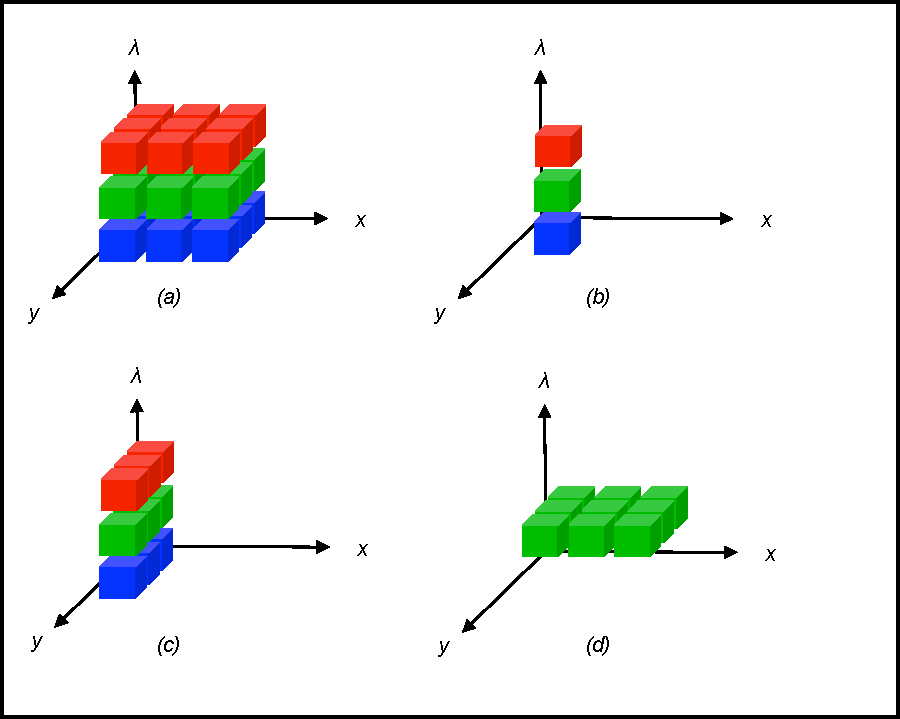
\includegraphics[scale=1.0]{isoCubes}
	\captionof{figure}[Discrete representation of the spectral datacube and various scanning measurement techniques]{(a) A discrete spectral datacube with $R_x = 3, R_y = 3, N_{\lambda} = 3$. (b) The whiskbroom technique measures the entire spectrum one spatial location at a time. (c) The pushbroom technique measures the entire spectrum on an entire spatial row or column at a time. (d) The tunable filter technique measurements an entire monochromatic image one spectral channel at a time.}
	\label{fig:isoCubes}
\end{figure}


The problem with the traditional ismorphic technique is that a typical spectral datacube has a significant amount of measurement samples. The \acrfull{aviris} system, acquires $R_x \times R_y = 677$ spatial locations (pixels) and $N_{\lambda} = 224$ spectral channels \cite{green1998imaging}, producing a spectral datacube with $N \approx 10^9$ measurement samples in $10$ minutes. 

Just like with the traditional spectrometer and camera, researchers have turned \gls{computational sensing} for spectral imaging. These architectures use the \gls{Fellgett advantage} (multiplexing) and \gls{Jacquinot advantage} (open aperture) to improve the \acrfull{snr} and reduce acquisition time and use a computational step to solve an inverse problem to reconstruct the spectral datacube \gls{spectralDataCube} from non-isomorphic measurements. Some spectral imaging architectures also leverage \gls{compressive sensing}. 

One of the early examples of computational sensing in spectral imaging is the \gls{ctis} \cite{descour1995computed}, see \Cref{fig:ctisArch}. The \gls{ctis} can reconstruct the spectral datacube \gls{spectralDataCube} from a single \gls{fpa} exposure by recording multiple measurements of the spectral datacube simultaneously. The \gls{ctis} uses several gratings to create two-dimensional projections of the three-dimensional hyperspectral datacube, see \Cref{fig:CTIS}. According to the central slice theorem, the two-dimensional Fourier Transform of each projection is a plane through the three-dimensional frequency space representation the spectral datacube. Ideally, one must collect enough projections to fully reconstruct the three dimensional frequency representation of the spectral datacube. The three-dimensional real-space distribution of the spectral datacube is then recovered through an inverse three-dimensional Fourier transform. This is similar to how computed tomography medical imaging works. However, in practice only a finite subset of projections are recorded and missing information is must be inferred. In the \gls{ctis}, the missing information is recovered by maximizing the likelihood of the measurement data using the expectation-maximization algorithm \cite{steven1993fundamentals, moon1996expectation}. According to the practical definition of compressive sensing, the \gls{ctis} maybe considered a compressive sensing technique since the number of measurement samples is less than the object dimensionality of the spectral datacube. However, it does not take advantage of sparsity or incoherence in order to reconstruct the spectral datacube.

\begin{figure}
	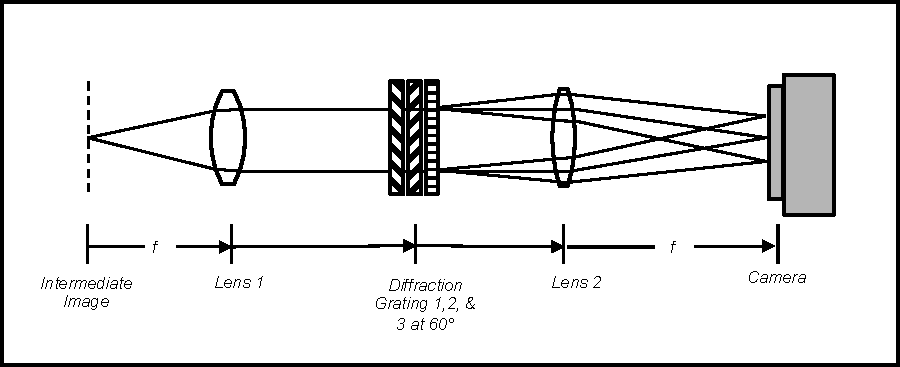
\includegraphics[scale=1.0]{ctisArch}
	\captionof{figure}[The architecture of the \acrfull{ctis}.]{The architecture of the \acrfull{ctis} consists of a collimating lens, several diffraction gratings, an imaging lens, and a \acrfull{fpa}. Each diffraction grating produces three two-dimensional projections of the three-dimensional spectral datacube (Two first order and one zeroth order). In this example,  gratings are rotationally seperated by 60 degrees to produce multiple projections. \cite{descour1995computed}}
	\label{fig:ctisArch}
\end{figure}

\begin{figure}
	\centering
	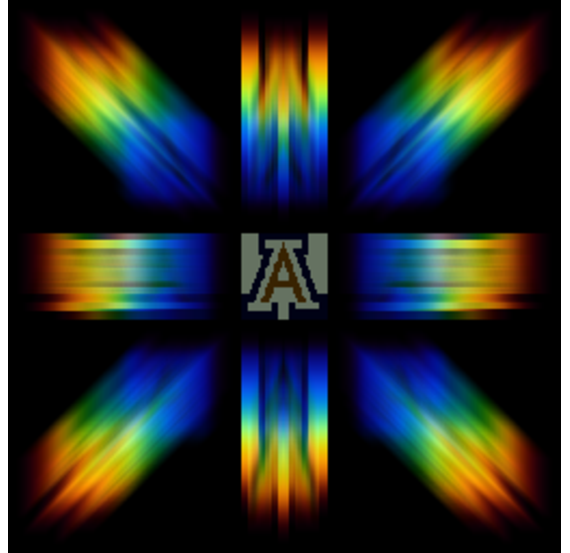
\includegraphics[scale=1.0]{CTIS.pdf}
	\captionof{figure}[The optical image before being sampled by the \gls{fpa} in the CTIS]{The optical image before being sampled by the \gls{fpa} in the \gls{ctis}. The \gls{ctis} uses multiple gratings to create projections of the spectral datacube at the \gls{fpa}. Note the center image is the zeroth order and is simply the undiffracted color image of the object scene \cite{descour1995computed}.}
	\label{fig:CTIS}
\end{figure}

In another example of computational sensing applied to spectral imaging is the \acrfull{cassi} sensor, see \Cref{fig:cassiArch}. In the \gls{cassi}, a coded aperture spatially codes the spectral datacube \gls{spectralDataCube}. The dispersive element then creates a projection of the spectral datacube that maps three-dimensional information into a two-dimensional image at the \gls{fpa}. Unlike the \gls{ctis}, only one two-dimensional projection is recorded per \gls{fpa} image which allows for higher spatial resolution for the same detector array. Using calibration data and prior knowledge of sparsity, the post-processing step solves the \gls{lasso} problem to reconstruct the spectral datacube \cite{wagadarikar2008single, arce2014compressive}. Often a total-variation regularization is also invoked to improve reconstruction of the spatially varying image \cite{wagadarikar2008spectral, bioucas2007new}.


\begin{figure}
	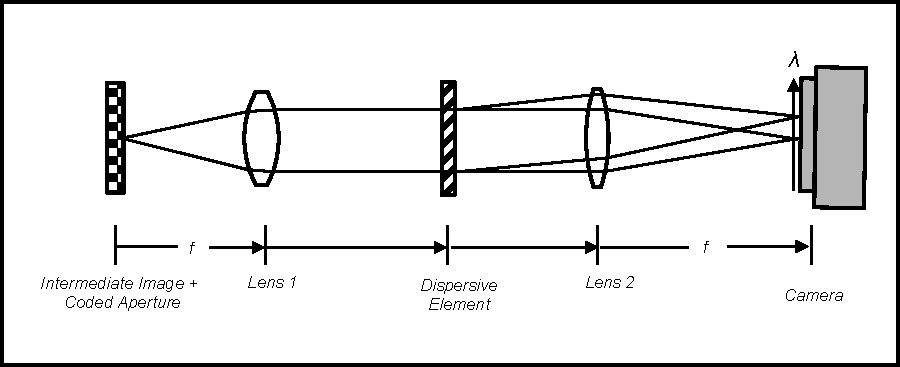
\includegraphics[scale=1.0]{cassiArch}
	\captionof{figure}[The architecture of the \acrfull{cassi}.]{The architecture of the \acrfull{cassi} consists of a collimating lens, a disperive element, an imaging lens, and a \acrfull{fpa}. The coded aperture spatially codes each wavelength layer in the three-dimensional spectral datacube. Then the dispersive element creates a wavelenght depedent spatial shift, shearing the spectral datacube. The monochromatic image of the \gls{fpa} creates a coded two-dimensional projection of the three-dimensional spectral datacube.}
	\label{fig:cassiArch}
\end{figure}


All traditional and computational spectral imaging architectures including the \gls{ctis} and the \gls{cassi} only reconstruct the spectral datacube \cite{hagen2013review}. This produces a significant amount of data, which is only used as an intermediate step. One is typically interested in determining the which chemical or material is responsible for a spectrum at a specific location. This is called spectral classification \cite{chang2003hyperspectral, dupont2011spatial, liu2014discriminative}. Therefore, an additional post-processing step needed. If however, one could directly classify the spectrum ,one could signficantly reduce the amount of data storage and communication resources required to operate the instrument. 

Previously my colleuges developed a computational spectrometer called the \acrfull{afss} \cite{dinakarababu2011adaptive}. Shown in \Cref{fig:afssArch}, the \gls{afss} was the first experimental computational sensor that make use of an adaptive scheme which uses measurement data to design spectral filters (codes). This allowed the spectrometer to directly classify the chemical or material responsible for the spectrum without the need to perform a reconstruction step. By combining the \gls{Fellgett advantage} with an adaptive algorithm to create custom spectral filters, the \gls{afss} was able to demonstate significant reduction in the number of measurements to classify a spectrum compared to non-adaptive multiplexed spectrometers in low \gls{snr} scenarios. In this context, the spectral filters act as feature vectors, which are computed using variation of \gls{pca}.\footnote{In the context of the AFSS and AFSSI-C the terms spectral filter, code, and feature vector are synonymous.}

The \acrfull{afssi-c} extends the concept first demonstrated by the \gls{afss} to spectral imaging. The \gls{afssi-c} directly classifies the spectrum at each spatial location without the need to reconstruct the spectral datacube. By adopting a task-specific sensing approach, the \gls{afssi-c} greatly improves classification accuracy while simultaneously reduces the amount of bandwidth and storage for data. Furthermore, the architecture of the \gls{afssi-c} leverages both the Fellgett and adaptive measurement scheme like the \gls{afss}, while also adding the Jacquinot advantag to outperform all traditional and currently known computational spectral imaging instruments in terms of number of measurements to correct classifcation.

\section{Architecture}

I want to quickly review the architecture of the \acrfull{afss} before discussing the architecture of the \gls{afssi-c}. The \gls{afss}, shown in \Cref{fig:afssArch}, is the earliest known computational spectrometer to use adaptive spectral filters to classify spectra \cite{dinakarababu2011adaptive}. Unlike the traditional slit spectrometer, the \gls{afss} images the dispersed slit onto a \gls{dmd}. The mirrors of the \gls{dmd} can then be adjusted to selectively reflect certain wavelengths towards the condensor lens, which then focuses light onto a single detector element \cite{dinakarababu2011adaptive}. By reflecting or ``turning on'' multiple \gls{dmd} mirrors and only using a single detector element, we achieved the \gls{Fellgett advantage}. By using measurement data to actively design spectral filters, the \gls{afss} outperforms non-adaptive schemes by eliminating spectra that improbable and turns it attention towards trying to classify the remaining high probability spectra. 

\begin{figure}
	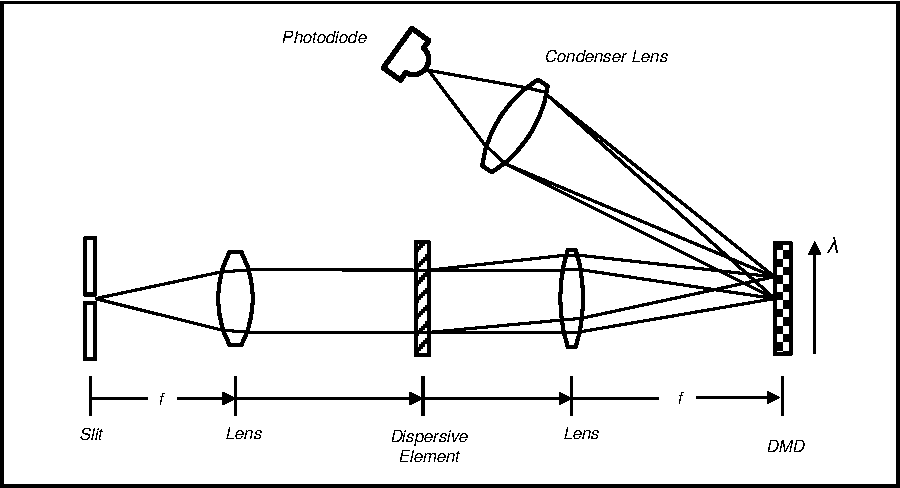
\includegraphics[scale=1.0]{afssArch}
	\captionof{figure}[The architecture of the Adaptive Feature Specific Spectrometer. ]{The slit blocks light from all but one spatial location. A lens collimates the light passed from the slit and a dispersive element creates monochromatic images of the slit at different columns on the \gls{dmd}, corresponding to different spectral channels. The \gls{dmd} can then selectively reflectives combinates of each spectral channels into the condenser lens. The condensor lens focuses all the light onto a single detector element, a photodiode.}
	\label{fig:afssArch}
\end{figure}

In order to create an imaging version of the \gls{afss}, one may naively attempt to extend the \gls{afss} architecture by forming a parallel array of \gls{afss} sensors to achieve classification across a spatial scene. However, just like in the proposed parallel single-pixel camera design in \Cref{chap:Scout}, this approach would significantly increase the \gls{swap-c} of the design. The \gls{afssi-c} provides a similar feature-based measurement approach and Bayesian framework but with a more compact architecture. Rather than a fully parallel version of the \gls{afss}, the optical design of the \gls{afssi-c} uses a single \gls{dmd} and a single set of lenses and dispersive elements sharing a common entrance pupil. This approach share resources across multiple spatial locations.


\begin{figure}
	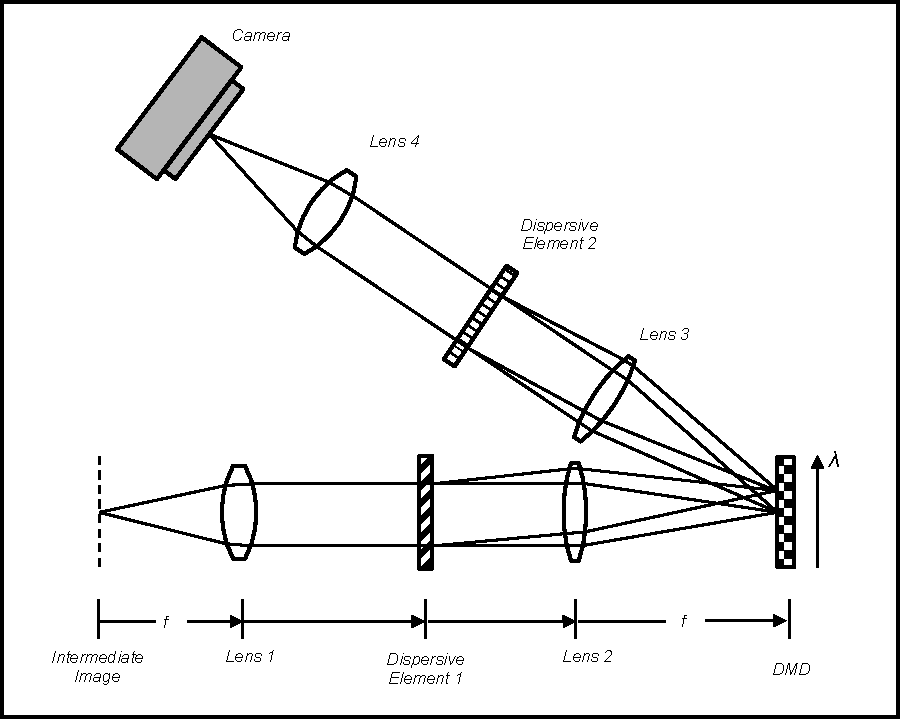
\includegraphics[scale=1.0]{afssicArch}
	\captionof{figure}[The architecture of the Adaptive Feature Specific Spectral Imaging-Classifier]{An objective lens forms the intermediate image of the object scene at the input plane of the instrument. The first lens collimates the light and a diffraction grating disperses the light. A second lens images spectrally dispersed versions of the image of the object scene onto the \gls{dmd}. The \gls{dmd} directs light to a beam dump or reflects the light towards the third lens on a mirror-by-mirror basis. Collimated light from third lens
is sent through a second grating, and finally imaged onto the detector by the fourth lens.}
	\label{fig:afssicArch}
\end{figure}


The design of the \gls{afssi-c} is essentially two 4\textit{f} open-aperture monochromators seperated by a \acrfull{dmd}, shown in Fig.~\ref{fig:afssicArch}. In our experiment, we used an objective lens, which is not shown, to create an intermediate image at the input plane of the instrument. At this point in the system one can imagine the source spectral datacube as depicted in \Cref{fig:sysCubes}(a), where $x$ and $y$ are the spatial axes, and $\lambda$ the spectral axis. The first lens of the system collimates the light from the input place. The first grating disperses the light. The second lens then images spectrally dispersed copies of the intermediate image on the \gls{dmd}. Just prior to being reflected from the \gls{dmd}, one can imagine the spectral dimension of the datacube as being sheared at an angle, in the direction of the dispersion, see \Cref{fig:sysCubes}(b). As in the \gls{afss}, each mirror on the \gls{dmd} either reflects light into the second arm or reflects light away into a beam dump (not shown). One can visualize this by looking at \Cref{fig:sysCubes}(c), a mirror that reflects light away, towards the beam dump, deletes columns in the sheared spectal datacube. The light that reflected into the second arm is then collimated before hitting the second grating, which is identical to the first, but with the reverse dispersion direction. This removes the shear in the encoded spectral datacube, seen in \Cref{fig:sysCubes}(d). Lens 4 images the unsheared spectral datacube onto the \gls{fpa}. The grayscale image of the \gls{fpa} essentially integrates the spectral datacube over the spectral dimension. 

\begin{figure}
	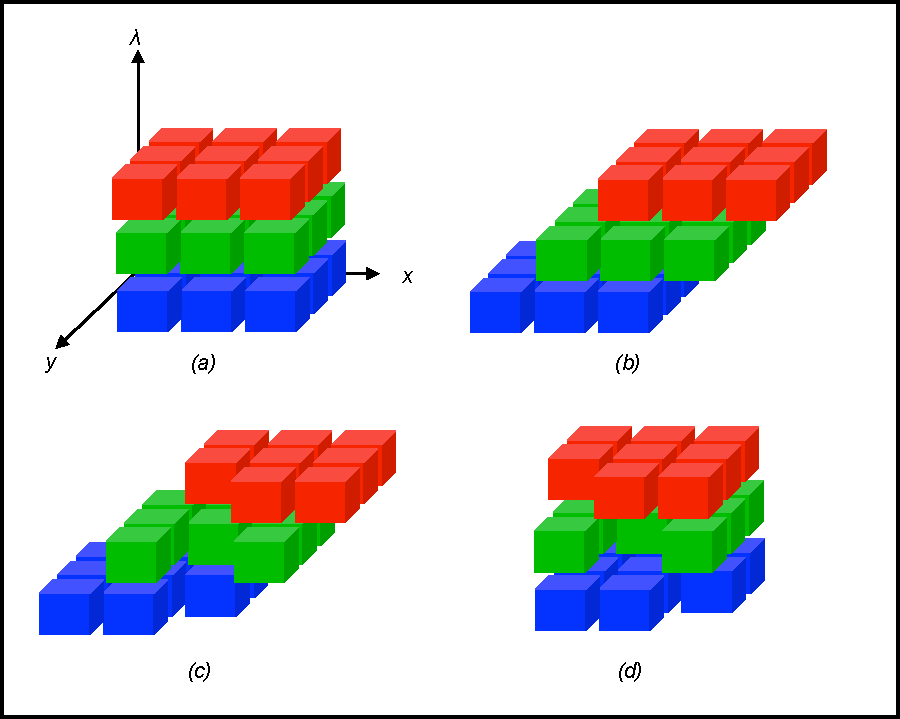
\includegraphics[scale=1.0]{justCubes}
	\captionof{figure}[Visualization of datacube progression through the \gls{afssi-c} system.]{(a) The input cube is (b) sheared by the first grating, (c) encoded at the \gls{dmd}, and finally (d) spatially re-registered by the second grating.}
	\label{fig:sysCubes}
\end{figure}

We choose to use a dual-disperser architecture rather than the single-disperser architecture such as the one in the \gls{cassi} since the mirror patterns on the \gls{dmd} acts as spectral filters for each spatial location. In the dual-disperser design, the spectral coding of each spatial location is more straightforward and elegant approach for parallel direct classification: the architectures allows us to write the image of each \gls{fpa} pixel as an innner product of the spectrum at the corresponding location at the source with the spectral filter created by the \gls{dmd}, allowing for parallel operation of the Bayesian inference approach. A single-disperser design would entangle both the spectral and spatial dimension of the spectral datacube, and would require solving a single larger joint inference problem.

\subsection{Forward Model}

Imagine a continuous spectral datacube which we call the source spectral density of $D_0 \left(x, y;\lambda \right)$ at the input aperture. To simplify the forward model analysis, assume unit magnification and ignore diffraction, aberrations, and vignetting. The spectral density just before reflection from the \gls{dmd} is written as:
%
\begin{equation}
\begin{split}
		D_1 \ap{ x, y; \lambda } & = \iint \delta \ap{x^\prime - \left[ x + \alpha \ap{\lambda - \lambda_c} \right] } \delta \ap{y^\prime - y } D_0 \ap{x^\prime, y^\prime; \lambda} dx^\prime dy^\prime \\
		& = D_0 \ap{x + \alpha \ap{\lambda - \lambda_c}, y; \lambda}
\end{split}
\end{equation}
%
Notice that this can thought of as a two-dimensional convolution of the spectral density with an wavelength dependant \acrfull{psf} that shifts the spectral density by an amount $\alpha \ap{\lambda - \lambda_c}$, where $\alpha$ is the dispersion and $\lambda_c$ is the center wavelength. If there is no dispersion, when $\alpha = 0$, then one would get the original spectral density back. Note, that when $\lambda = \lambda_c$ there is no shift in the $x$ direction. 

After reflecting from the \gls{dmd} the spectral density can then be written as:
%
\begin{equation}
D_2 \ap{ x, y; \lambda } = T\left( x, y \right) D_1\ap{ x, y; \lambda} = T \ap{ x, y } D_0 \ap{x + \alpha \ap{\lambda - \lambda_c}, y; \lambda}
\end{equation}
%
where $T \ap{ x, y }$ represents the reflection pattern of the \gls{dmd}. If $T = 1$ the light is being reflected into the second arm and if $T = 0$ the light is being reflected towards the beam dump. 

Propagating through the second arm has the effect of reversing the shear imposed on the spectral density:
%
\begin{equation}
\begin{split}
	D_3 \ap{x,y;\lambda} & = \iint  \delta \ap{x^\prime - \left[ x - \alpha \ap{\lambda - \lambda_c} \right]} \delta \ap{y^\prime - y} D_2 \ap{x,y;\lambda} dx^\prime dy^\prime \\
	& = T \ap{x - \alpha\ap{\lambda - \lambda_c},y} D_0 \ap{x,y;\lambda} \\
	& = H \ap{x,y;\lambda} D_0 \ap{x,y;\lambda}
	\label{eq:afssicFilter}
\end{split}
\end{equation}
%
Notice that the dispersion $\alpha$ has the opposite sign. This equation is represented in discrete form in \Cref{fig:sysCubes}(d). Thus, propating through the entire optical system represents multiplying the input spectral density with a spectral desnity filter function $H \ap{x,y;\lambda}$. 

Since the \gls{fpa} image is grayscale, ignoring quantization effects, the image can be written as an integral over the wavelengths
%
\begin{equation}
	I\ap{x,y} = \int H \ap{x,y;\lambda}  D_0 \ap{x,y;\lambda} d\lambda
\end{equation}
%
By taking into account the spatially pixeled detector array with pixel size $\Delta$, then the discrete \gls{fpa} image is
%
\begin{equation}
	\Gamma_{nl} = \iiint \mbox{rect} \ap{ \frac{x}{\Delta} - n, \frac{y}{\Delta} - l } H \ap{x,y;\lambda} D_0 \ap{x,y;\lambda} dx^\prime dy^\prime d\lambda
	\label{eq:afssicDiscreteReadout}
\end{equation}
%
where $\Gamma_{nl}$ is the image value from the $n^{th}$ and $l^{th}$ location. Now consider that the \gls{dmd} pattern $T$ is also pixelated with the same pixel size $\Delta$ as in the detector. 
%
\begin{equation}
	T \ap{x,y} = \sum_{n^\prime, l^\prime}  T_{n^\prime, l^\prime} \mbox{rect} \ap{ \frac{x}{\Delta} - n^\prime, \frac{y}{\Delta} - l^\prime}
	\label{eq:afssicDiscreteDMD}
\end{equation}
%
Inserting \Cref{eq:afssicDiscreteDMD} into \Cref{eq:afssicFilter} and \Cref{eq:afssicDiscreteReadout} produces a single equation which describes how the signal-of-interest $D_0 \left( x, y; \lambda \right)$ is measured by the \gls{afssi-c}:
%
\begin{align} \label{eq:PixelizedDetectIntensity}
	\Gamma_{nl} &= \sum_{n^\prime l^\prime} \iiint \mbox{rect} \left( \frac{x}{\Delta} - l, \frac{y}{\Delta} - n \right) \mbox{rect} \left( \frac{x-\alpha \left(\lambda - \lambda_c\right)}{\Delta} - l^\prime , \frac{y}{\Delta} - n^\prime \right) \notag \\
 	&\qquad \times T_{n^\prime l^\prime} D_0 \left( x, y; \lambda \right) dx \, dy \, d\lambda.
\end{align}
%
This equation maybe somewhat difficult to interpret, so to add some additional intuition I will go through an example of a monochromatic source at the center wavelength, $D_0 \left(x, y, \lambda\right) = I_0 \left(x, y \right) \delta \left( \lambda - \lambda_c \right)$, where $I_0$ is the intensity distribution of the monochromatic scene. In this case, \Cref{eq:PixelizedDetectIntensity} simplifies to
%
%
\begin{align} \label{eq:MonoChrome}
	\Gamma_{nl} \left(\lambda = \lambda_c \right) &= \sum_{ n^\prime l^\prime} \iiint \mbox{rect} \left( \frac{x}{\Delta} -  l, \frac{y}{\Delta} - n \right)  \mbox{rect} \left( \frac{x}{\Delta} - l^\prime, \frac{y}{\Delta} - n^\prime \right) \notag \\
	&\qquad \times T_{n^\prime l^\prime} I_0 \left( x, y \right) \delta \left( \lambda - \lambda_c \right) dx \, dy \, d\lambda  \notag \\
	%
	&= \sum_{ n^\prime l^\prime} T_{n^\prime l^\prime}  \iint \mbox{rect} \left( \frac{x}{\Delta} -  l, \frac{y}{\Delta} - n \right)  \mbox{rect} \left( \frac{x}{\Delta} - l^\prime, \frac{y}{\Delta} - n^\prime \right) \notag \\
	&\qquad \times I_0 \left( x, y \right) dx \, dy \, \int \delta \left( \lambda - \lambda_c \right)d\lambda  \notag \\
	%
 	&= \sum_{n^\prime l^\prime} \delta_{ll^\prime} \delta_{nn^\prime} T_{n^\prime l^\prime} I_{nl} \notag \\
 	&= T_{nl} I_{nl},
\end{align}
%
where $I_{nl}$ is a spatially pixelated version of the monochromatic source with intensity distribution $I_0 \left(x, y \right)$. One now sees that in the monochromatic case, the measurement is point-by-point multiplication of the \gls{dmd} pattern with the discrete monochromatic image $I_{nl}$

In the next example, I consider the case where a monochromatic source is not at the center wavelength but is shifted in wavelength. The wavelength of the monochromatic source is shifted from the center wavelength by a single spectral channel $\lambda= \lambda_c + \Delta_{\lambda}$, where $ \Delta_{\lambda} = \Delta / \alpha$. The spectral density is now written as $D_0 \left(x, y, \lambda\right) = I_0 \left(x, y \right) \delta \left( \lambda - \ap{\lambda_c + \Delta_{\lambda} } \right)$. \Cref{eq:PixelizedDetectIntensity} simplifies to
%
\begin{align} 
	\Gamma_{nl}\left(\lambda = \lambda_c + \Delta \lambda\right) &= \sum_{n'l'} \iiint \mbox{rect} \left( \frac{x}{\Delta} - l, \frac{y}{\Delta} - n \right)  \mbox{rect} \left( \frac{x}{\Delta} - \left(l' + 1 \right), \frac{y}{\Delta} - n' \right) \notag \\
 	&\qquad \times T_{n'l'} I_0 \left( x, y \right) \delta \left( \lambda - \left( \lambda_c + \Delta \lambda \right)\right) dx \, dy \, d\lambda  \notag \\
 	%
	&= \sum_{ n^\prime l^\prime} T_{n^\prime l^\prime}  \iint \mbox{rect} \left( \frac{x}{\Delta} -  l, \frac{y}{\Delta} - n \right)  \mbox{rect} \left( \frac{x}{\Delta} - \left(l' + 1 \right), \frac{y}{\Delta} - n' \right) \notag \\
	&\qquad \times I_0 \left( x, y \right) dx \, dy \, \int \delta \left( \lambda - \left( \lambda_c + \Delta \lambda \right)\right) d\lambda  \notag \\
	%
 	&= \sum_{n'l'} \delta_{l \left( l' + 1 \right) } \delta_{nn'} T_{n' l'} I_{nl} \notag \\
 	&= T_{n\left(l - 1 \right)} I_{nl}
 	\label{eq:Mono2}
 \end{align}
%
This shows that a shift by one spectral channel results in a shift of one pixel in of the \gls{dmd} pattern.

Using the intuition from the last two examples, I will now extend this to a non-monochromatic case. Consider spectral channel index \gls{specchan} out of \gls{numspecchan} total spectral channels.
We can also define a discretized source spectral datacube $D_{nlc}$, and then the detector signal $\Gamma_{nl}$ as a result of mirror pattern $T$ acting on the pixelated source is
%
%
\begin{equation}
	\Gamma_{nl} = \sum^{N_{\lambda}-1}_{c = 0} T_{n \left( l + c \right)} S_{nlc},
\end{equation}
%
%
which shows the measurement at each pixel being the inner product of the source spectrum and the spectral filter which results from the mirror pattern. If one inspects the adjacent pixel on the detector, $\Gamma_{n \left(l +1 \right)}$ we find that
%
%
\begin{equation}
\Gamma_{n\left(l-1\right)} = \sum^{N_{\lambda}-1}_{c = 0} T_{n\left( l + 1 + c \right)} S_{n\left(l+1\right)c}.
\end{equation}
%
%
The spatial location $\left(n,l \right)$ sees the effect of the pattern in mirror locations $T_{nl}$ to $T_{n\left(l+N_{\lambda}-1\right)}$, while the neighboring spatial location at $n, \left( l + 1\right)$ is encoded by the mirror pattern from $T_{n\left(l+1\right)}$ to $T_{n\left(l + N_{\lambda} \right)}$. Notice that given two neighboring spatial pixels in the input aperture, $l$ and $l+1$, mirror pixels $T_{n\left( l + 1 \right)}$ to $T_{n\left(l + N_{\lambda} - 1 \right)}$ are common to both locations. 

Now the design constraint of the \gls{afssi-c} architecture is clear, while a naively parallel set of \gls{afss} would have been costly in terms of \gls{swap-c}, using a common entrance pupil prevents indepdent spectral filters for each spatial location. The spectral filters imposed by the \gls{dmd} pattern maybe unique for every spatial location, but \textit{cannot} be implemented independently, requiring the features to be designed \textit{jointly} for spatial locations along a row (the $l$ direction).



\section{Adaptive Classification Algorithm}

As mentioned earlier, the \gls{afssi-c} uses adaptive features to directly classify the spectrum at each spatial location. At each measurement step $m$, the classification algorithm computes the probability of each hypothesis spectra in a spectral library. Building on the discussion of \acrfull{pca} and Bayesian statistics in \Cref{chap:Formalism}, I will discuss how the classification algorithm of the \gls{afssi-c} works. 


Since the \gls{afssi-c} feature vectors are not indpendent for each spatial location, it is more intuitive to discuss the algorithm when only a single spatial location exist in the spectral datacube. The reader can then expand the intuition to the entire scene. For a single pixel architecture, one can write the discrete forward model as
%
\begin{equation}
g_m = \mb{t}_{m}^{T} \mb{f}
\end{equation}
%
where $g_m$ is the $m^{th}$ measurement of \gls{dmd} mirror pattern $\mb{t}_m$ and $\mb{f}$ is the ground truth spectrum of the source. 

The measurement from the detector is compared to the spectral library, subject to the spectral filter implemented at that spatial location. A probability is assigned to each hypothesis in the spectral library using Bayes' theorem. The conditional probability of the hypothesis, which is spectrum $\mb{s}_i$ is present, given the measurement history up to the $m^{th}$ measurement $\{g\}_m$, can be written as:
%
\begin{equation}\label{eq:BayesThm2}
\mbox{P} \left( h_i | \{ g \}_m \right) = \frac{\mbox{P} \left( \{g\}_m |\, h_i \right) \; \mbox{P} \left(h_i\right)}{\mbox{P} \left( \{g\}_m \right)}.
\end{equation}



Remember from Chapter 2, that \gls{pca} provides the optimal basis to distinguish between data vectors in a vector space by diagonalizing the covariance matrix. The covariance matrix (or scatter matrix) is simply the matrix multiplication of the spectral library (with the mean spectrum subtracted) with the transpose of itself. 

\begin{align}
\textbf{Q} &= \sum^{N_{R}}_{r \;= \,1} \left(\textbf{s}_r - \bar{\textbf{s}} \right) \left(\textbf{s}_r - \bar{\textbf{s}} \right)^T \notag \\
&=\textbf{X}\;\textbf{X}^T. \label{eq:nonweightedScatter}
\end{align}

However, since the spectral library is constant with respect to the measurements, the set of principal components will also remain constant. Intuitively, one can use the probability of each spectrum that was computed from the last measurement to weight each of the spectra in the library. Geometrically, one can imagine that the direction of largest variation is now biased to align in the direction with higher probability spectra. The geometric depiction of the probabilistically weighted \acrfull{pca} which we call pPCA is shown in \Cref{fig:pPCA}.

%
\begin{figure}[htb]
  \centering
  % Requires \usepackage{graphicx}
  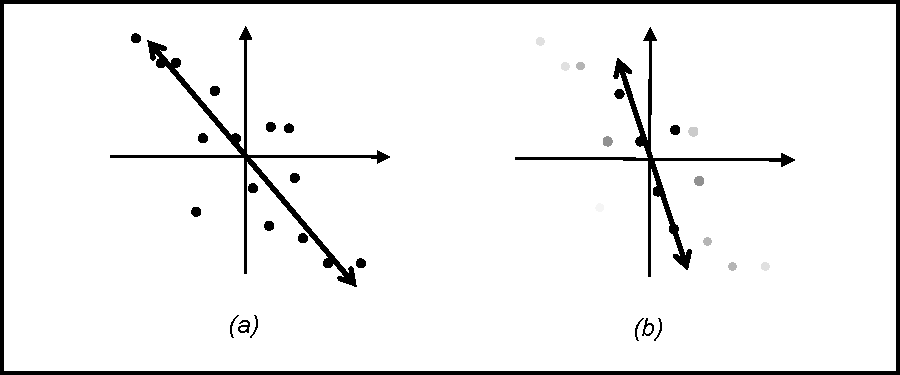
\includegraphics[scale=1.0]{pPCA}
  \caption{Depiction of the pPCA (simple 2D example). (a) First principal component before a measurement has been made. All of the hypotheses are equiprobable, depicted here as all points having the same grayscale value. (b) After a measurement has been made: the darker points are more probable hypotheses, with the less probable hypotheses taking on lighter shades of gray. The first principal component has now been shifted to the direction of greatest variation in the weighted data.}\label{fig:pPCA}
\end{figure}
%
I will now go over the formalism for \gls{ppca}. At each spatial location, we create a covariance matrix with \gls{numspeccand} spectral hypotheses, with individual spectrum $\textbf{s}_r$, weighted in relation to the prior probability associated with each hypothesis given the measurement history. The individual covariance matrices $\textbf{{Q}}(m)$ at each spatial location with spectral library element hypothesis $h_r$ take the form
%
%
\begin{align}
\textbf{Q}(m) &= \sum^{N_{\lambda}}_{r \;= \,1} \mbox{P} \left( h_r | \{g\}_m \right) \left(\textbf{s}_r - \bar{\textbf{s}} \right) \left(\textbf{s}_r - \bar{\textbf{s}} \right)^T \notag \\
&=\textbf{X}(m)\;\textbf{X}^T(m). \label{eq:preScatter}
\end{align}
%
%
Here $\textbf{X}(m)$ is the matrix of weighted spectral elements, where the row index $i$ is from 1 to the number of spectral channels $N_{\lambda}$; the columns $r$ from 1 to \gls{numspeccand} as follows,
%
%
\begin{equation}
	\textbf{x}_{r}(m) = \sqrt{\mbox{P} \left(h_r \vert \{g\}_m \right)} \left(\mb{s}_{r} - \bar{\textbf{s}}\right),
\end{equation}
%
%
and $\bar{\textbf{s}}$ is the probabilistically-weighted sum of the spectral library:
%
%
\begin{equation} \label{eq:Sbar}
\bar{\textbf{s}} = \sum^{N_R}_{r \;= \, 1} \mbox{P} \left( h_r | \{g\}_m \right) \textbf{s}_r.
\end{equation}


We can then compute the first eigenvector of $\textbf{Q}(k)$, analogous to PCA. We call this probabilistic-PCA or pPCA, and in the case of the AFSS this eigenvector becomes the feature for the next measurement. The scatter matrix $\textbf{Q}(k)$ is then updated with every measurement.

\subsection{Updating Probabilities}\label{ssec:updatingProbabilities}

In practice we do not directly compute the posterior probabilities for each hypothesis using Bayes' theorem, \Cref{eq:BayesThm2}, since we have no meaningful way of computing the probability of the measurement history $\prob{ \{g\}_m }$. Thankfully, the method of \acrfull{map} and taking ratios of posterior probabilities that I discussed in Chapter 2 allows one to compute relative probabilities which will be used to weight the spectral library after each measurement. For now I will define the ratio of the posterior probabilities
%
\begin{equation}
	  L_{ij}^{\left\{ g \right\}_m} := \pr{h_i | \{g\}_{m} }{h_j | \{g\}_{m} } = \pr{ \{g\}_{m}|h_i }{ \{g\}_{m}|h_j} \pr{h_i}{h_j}
	  \label{eq:initRatio1}
\end{equation}
%
where $\{g\}_{m}$ is the set of all measurements, including the current measurement number index $m$.


Note that if we assume that the likehood probabilities are indepdent, then we can write the joint probability as a product of the likelihood of the current measurement with the likelihoods of all past measurements
%
\begin{align}
	\prob{\{g\}_m|h_i} &= \prob{g_m|h_i} \prob{\{g\}_{m-1}|h_i} \notag \\
							&= \prob{g_m|h_i} \prod_{m'=1}^{m-1} \prob{g_{m'}|h_i}
\end{align}
So we can expand \Cref{eq:initRatio1} 

\begin{equation}
	  L_{ij}^{\left\{ g \right\}_m} =  \frac{ \prob{g_m|h_i} \prod_{m'=1}^{m-1} \prob{g_{m'}|h_i} }{ \prob{g_m|h_i} \prod_{m'=1}^{m-1} \prob{g_{m'}|h_j}} \pr{h_i}{h_j}
	  \label{eq:initRatio2}
\end{equation}
%
If I define
%
\begin{equation}
L_{ij}^{\left\{ g \right\}_{m-1}} := \frac{ \prod_{m'=1}^{m-1} \prob{g_{m'}|h_i} }{ \prod_{m'=1}^{m-1} \prob{g_{m'}|h_j}} \pr{h_i}{h_j}
\end{equation}
%
then \Cref{eq:initRatio2} simplifies into
%
\begin{equation}
	  L_{ij}^{\left\{ g \right\}_m} =  \frac{ \prob{g_m| h_i} } { \prob{g_m| h_j} } L_{ij}^{\left\{ g \right\}_{m-1}}
	  \label{eq:initRatio3}
\end{equation}
%
This equation provides a convient way to update the ratio of posterior probabilities after each measurement.

The question now turns to how does one actually compute the likelihoods. For this step we assumed that the likelihood takes on a Gaussian noise model with standard deviation of the noise $\sigma_{\text{AWGN}}$. Thus we say the probability of the measurement $g_m$ given that hypothesis $h_i$ is true is 
%
\begin{equation}
	\prob{g_m | h_i } = \frac{1}{\sqrt{2\pi\sigma_{\text{AGWN}}^2 }} 
	\exp \left[ - \frac{ \ap{g_m - \mb{t}_m \cdot \mb{s}_i } }{2 \sigma_{\text{AGWN} }^2} \right]
	\label{eq:noiseModel1}
\end{equation}
%
where $\mb{t}_m$ is the spectral filter at the measurement step $m$. This equation means that when the measurement value $g_m$ is close to the inner product of the spectral filter and the hypothesis spectrum, the probability is large. As the measurement value deviates from $\mb{t}_m \cdot \mb{s}_i $ the probability decreases.

After each measurement we compute \Cref{eq:initRatio3} for all pairs of spectra ${i,j}$ using the noise model \Cref{eq:noiseModel1}. In practice, the exponentials of numbers of moderate size cause numerical issues. To avoid this, we compute the logarithm of the likelihood (log-likelihood) ratios to eliminate the exponentials. In Appendix \ref{app:Derivation of the LLR Update}, I will discuss the update rule using log-likelihood ratios. 

\subsection{Extension to Spectral Imaging}

In the case of spectral classification for only a single spatial location, like the \gls{afss}, the number of \gls{dmd} mirrors is equal to the number of spherical channels. 
%
\begin{equation}
	N_d = N_{\lambda} 
\end{equation}
%
As we saw before the dimensionality of the feature vectors produced by taking the eigenvectors of the covariance matrix is equal to the number of spectral channels. 

In the \gls{afssi-c} architecture, light from spatial pixel $l$ is dispersed onto DMD pixels $l$ to $l + N_{\lambda} - 1$. While light from the next spatial pixel $l + 1$, is dispersed onto DMD pixels $l + 1$ to $ \ap{l + N_{\lambda}} $. Therefore adjacent spatial pixels have $N_{\lambda} - 1$ DMD pixels in common. Light is not dispersed between rows. This means that one can treat the design of the features between different rows seperately. However, within a particular row, this dispersion constrains our ability to indepdently design features to classify the spectral for each spatial location on the row. This is one of the major design constraints in the \gls{afssi-c}. 

It turns out, one can still use pPCA by constructing a very large data matrix $\tilde{\mathbf{X}}$. The individual probabilistically weighted spectral library matrices $\mb{X}_l$ for each spatial pixel $l$ is placed inside $\tilde{\mathbf{X}}$. The adjacent spatial location will have $\mb{X}_{l+1}$ placed next to it but one row down. The first row is padded with zeros. 

For example, imagine two adjacent spatial pixels $l = 1$ and $l = 2$ with five spectral channels $N_{\lambda} = 5$ and three spectra in the spectral library $N_R = 3$.
\begin{equation}
\tilde{\mathbf{X}} =
\begin{bmatrix}
    x_{1,1,1}  & x_{1,2,1} & x_{1,3,1} 	& 0 	    & 0 		& 0 \\
    x_{2,1,1}  & x_{2,2,1} & x_{2,3,1} 	& x_{1,1,2} & x_{1,2,2} & x_{1,3,2} \\
    x_{3,1,1}  & x_{3,2,1} & x_{3,3,1} 	& x_{2,1,2} & x_{2,2,2} & x_{2,3,2} \\
    x_{4,1,1}  & x_{4,2,1} & x_{4,3,1} 	& x_{3,1,2} & x_{3,2,2} & x_{3,3,2} \\
    x_{5,1,1}  & x_{5,2,1} & x_{5,3,1} 	& x_{4,1,2} & x_{4,2,2} & x_{4,3,2} \\
    0		   & 0	       & 0      			& s_{5,1,2} & s_{5,2,2} & s_{5,3,2} 
\end{bmatrix}
\end{equation}
%
The subscripts of element $x_{c,r,l}$ refer to $c$ the spectral channel, the $r^{th}$ spectrum in the spectral library and $l$ the spatial pixel index. Therefore we see that the first three columns are just $\mb{X}_1$, the modified spectral library for spatial pixel $l=1$ and the last three columns is the modified spectral library $\mb{X}_2$ for spatial pixel $l = 2$.

Notice that the rows of this matrix have physical meaning. The first row corresponds to the first \gls{dmd} pixel, since only spectral channel one from all three possible spectra from location $l = 1$ can be imaged onto the first \gls{dmd} pixel (mirror). The second row corresponds to the second spectral channel of the three possible spectra from location $l = 1$ and the first spectral channel of the three possible spectra from location $l = 2$.  

The revised covariance matrix is now

\begin{equation}
\tilde{\mathbf{Q}} = \tilde{\mathbf{X}} \tilde{\mathbf{X}}^{T}
\end{equation}
%
Where $\tilde{\mathbf{X}}^{T}$ is the transpose of the matrix $\tilde{\mathbf{X}}$. Thus the columns of $\tilde{\mathbf{X}}^{T}$ have the same physical interpretation as the rows of $ \tilde{\mathbf{X}}$. Each element of $\tilde{\mathbf{Q}}$ is therefore the covariance of each of the possible spectral channel from each location onto each \gls{dmd} mirror. Thus pPCA is computing the eigenvector of the covariances in the ``DMD mirror space''. This is what we call the joint-pPCA, basically the extension of pPCA to the imaging problem.  


% joint-pPCA figure
%\begin{figure}[htb]
%	\centering
%	\includegraphics[height=3.0in]{jointpPCA}\\
%	\caption{Joint-pPCA schematic. (a) The pictorial illustration of the formation of $\textbf{X}(k)$ from Equation(\ref{eq:preScatter}). The hypothesis spectra (1) are centered around the mean (2), and given a weight based on their probabilities (3).  (b) The joint-pPCA calculation involves the stacking of the $1, \ldots, C-1$ elements of $\textbf{X}_{i, j}(k)$ for each location $\left( n^\prime,\;l^\prime \right)$ along a row into a larger matrix $\textbf{\~X}_{uv}(k)$. The final joint-pPCA scatter matrix is formed from $\textbf{\~X}(k)$ multiplied by its mean-centered transpose, to arrive at scatter matrix $\textbf{\~Q}(k)$. The first principal component of this much larger scatter matrix is then in the direction of greatest variation in the joint-position data.}\label{fig:jointpPCA}
%\end{figure}
\clearpage


\section{Experiments}

A systems level flowchart is shown in \Cref{fig:afssicFlowchart} which shows each of the major steps in running the \gls{afssi-c} experiment. In this section, I will discuss each step, with the goal of continuing to concentrate on the practical considerations of the \gls{afssi-c}. The experimental results in this dissertation are for a 4-class problem, with an input spectral datacube of 64 $\times$ 64 spatial pixels and 38 spectral channels. \Cref{fig:afssicSpecLib} and \Cref{fig:afssicUofAsource} are depictions of the associated 4-class spectral library, with the spectral source displayed on the LED monitor. While this spectral datacube is small compared to those used in remote sensing, the implemented size was driven by practical considerations regarding the source, \gls{dmd} and detector on hand. The dual-disperser architecture, in general, places no significant limitation on possible datacube sizes. Similarly, the processing involved in the Bayesian inference and feature design are computationally lightweight and do not create a computational limit on datacube size.

% joint-pPCA figure

\begin{figure}[h!]
	\centering
	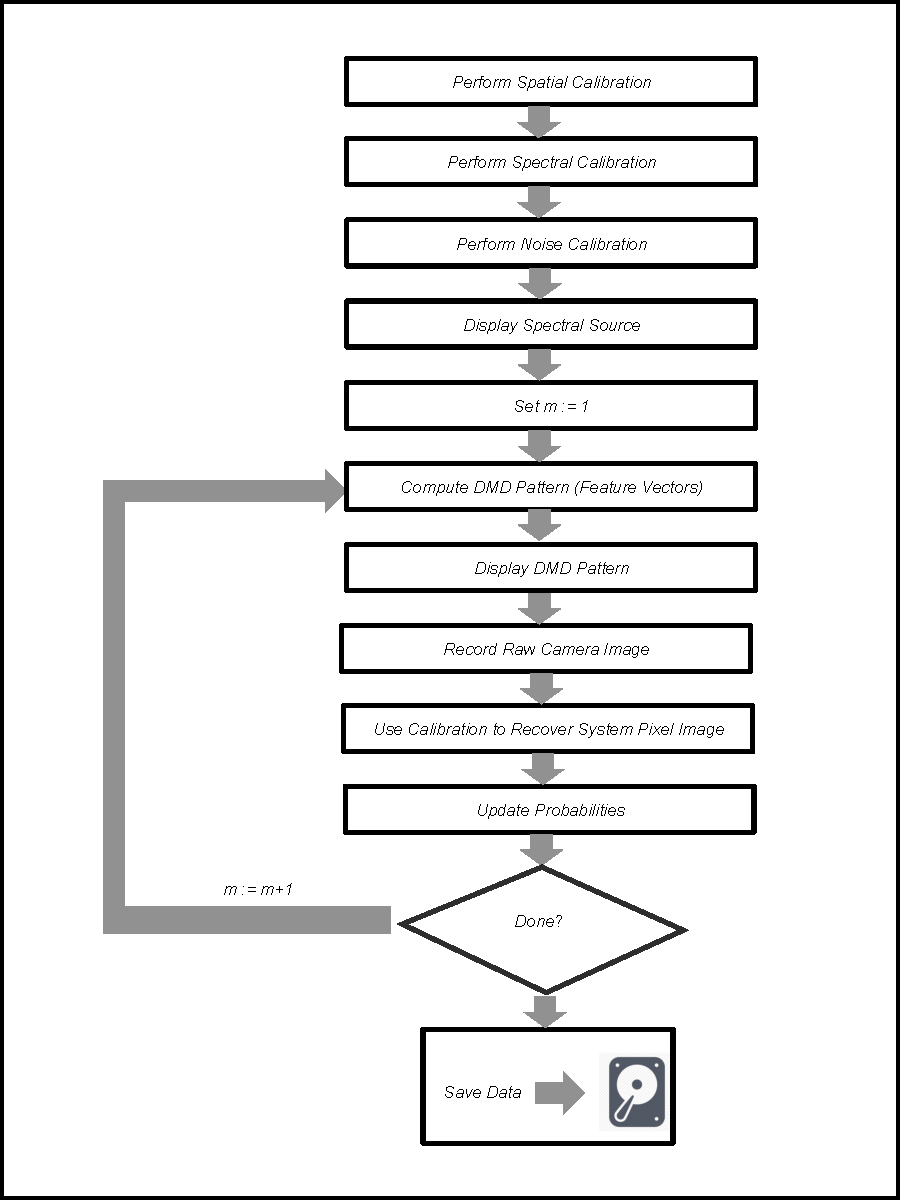
\includegraphics[scale=1.0]{afssicFlowchart}\\
	\captionof{figure}[Systems Level Flowchart for AFSSI-C Experiment]{Systems Level Flowchart of the AFSSI-C Experiment}
	\label{fig:afssicFlowchart}
\end{figure}


Classification difficulty is quantified as the \acrfull{tsnr} which considers the noise in the system relative to the separation distance between hypotheses spectra. We define \gls{tsnr} as
%
\begin{equation}
\text{TSNR} = 10 \log_{10} \ap{ \frac{d_{min}}{\sigma} }
\end{equation}
%
For our experiment, the noise is approximately \gls{awgn} distributed with standard deviation $\sigma$. The minimum Euclidean distance between the hypotheses in the spectral library $d_{min}$. When using this definition for TSNR, a value of 0 dB TSNR is the point where the noise is equal to the minimum distance between the library elements.


% Plot of the \gls{afssi-c} 4 Class Spectral Library
\begin{figure}[htb]
	\centering
	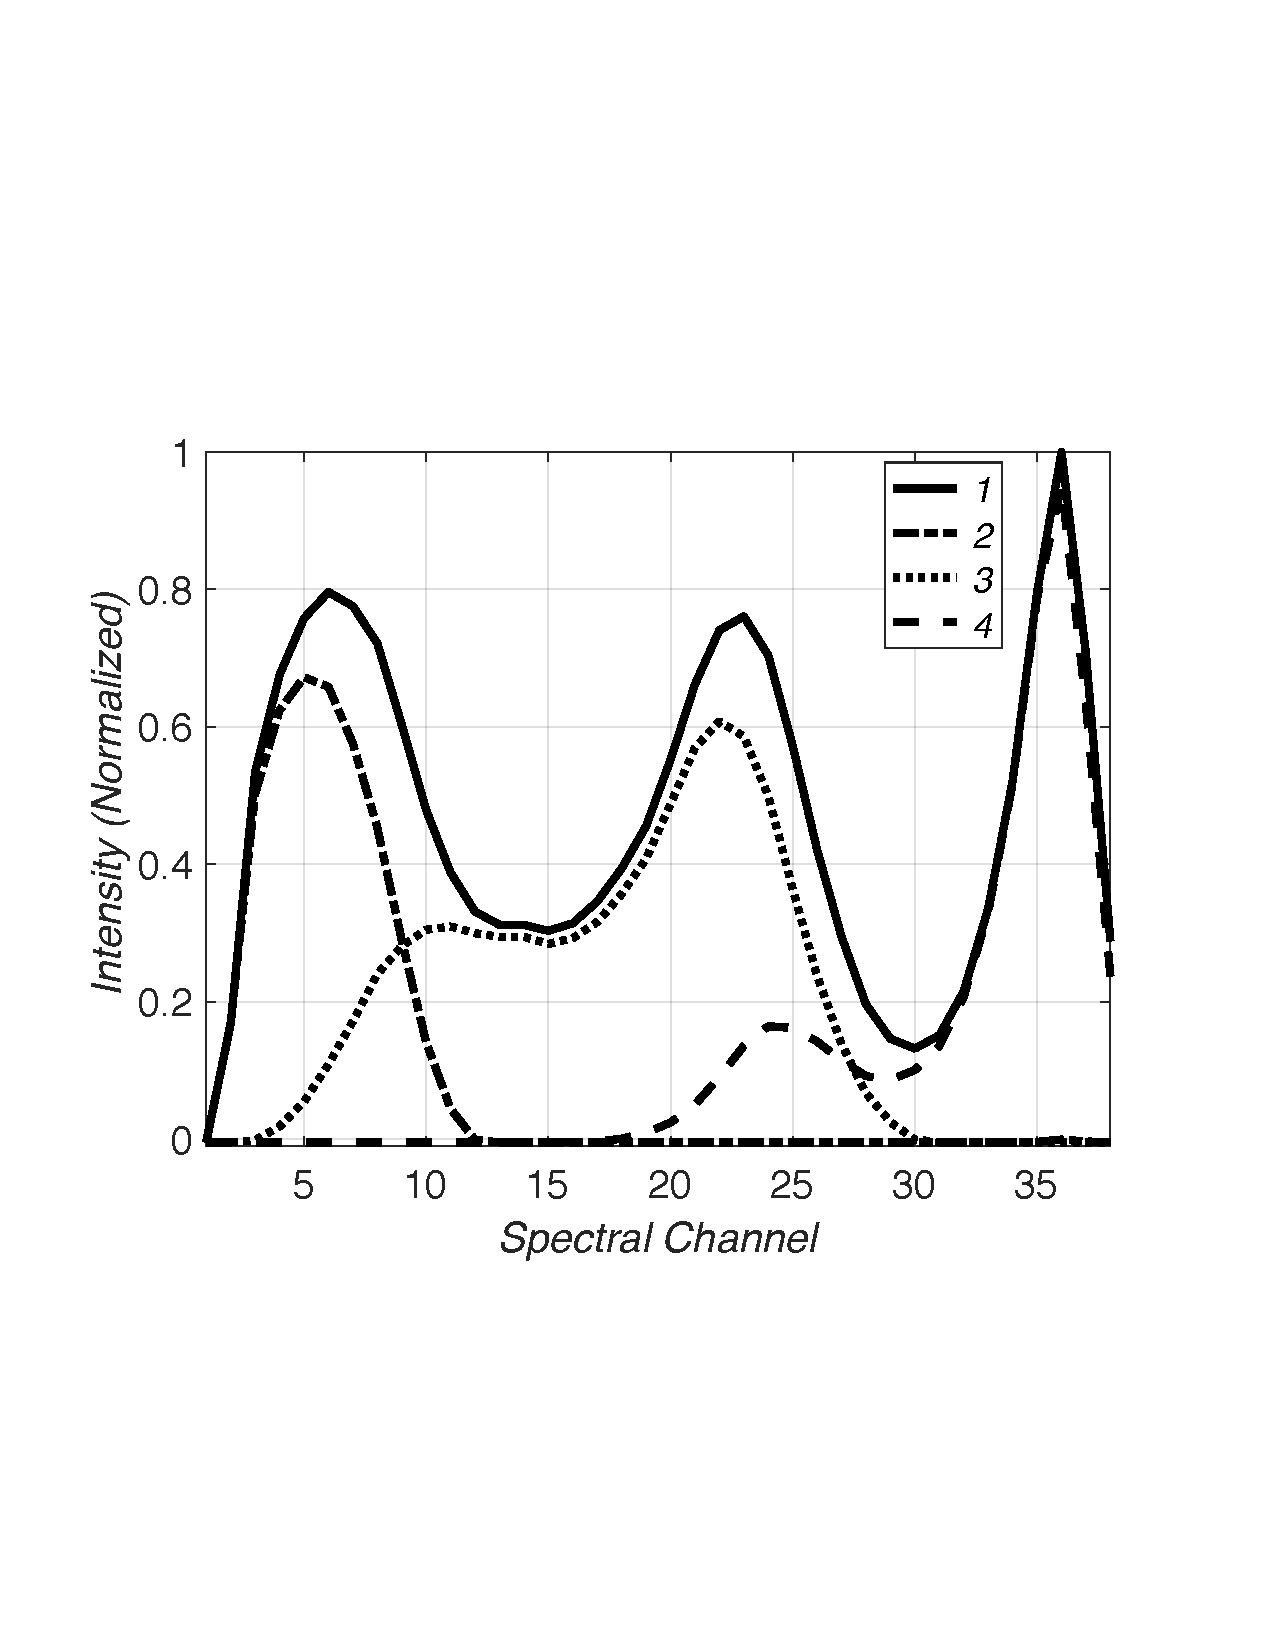
\includegraphics[scale=0.845]{afssicSpecLib}\\
	\captionof{figure}[Four class spectral library used for the AFSSI-C experiment.]{The spectral library consists of four spectral classes: the white, red, green, and blue of the LED monitor.}
	\label{fig:afssicSpecLib}
\end{figure}


% Plot of the UofA Symbol
\begin{figure}[htb]
	\centering
	
\includegraphics[scale=0.90]{afssicUofAsource}\\
	\captionof{figure}[Four class spectral source used for the \gls{afssi-c} experiment]{Four class spectral source used for the AFSSI-C experiment.}
	\label{fig:afssicUofAsource}
\end{figure}

\subsection{Hardware}

I will now discuss the hardware used in the \gls{afssi-c} experiment, shown in \Cref{fig:afssicPhoto1}. Specifically I will describe some of the design decisions and consequences of those decisions in the \gls{afssi-c} experiment. To avoid expensive and time consuming optical design and fabrication, the lenses were restricted to commercial off-the-shelf achromatic doublets. A compact, fixed focal length, lens (Edmund Optics Stock No. 58-001, f = 12mm) is used as an objective lens, relaying the object onto an intermediate image plane. A fast entrance optic is needed to meet the layout and magnification requirements. Referring to \Cref{fig:afssArch}, lenses 1 and 4 are 75 mm focal length achromatic doublets with a 50 mm diameter (Edmund Optics Stock No. 49-291), and lenses 2 and 3 are 150 mm focal length achromatic doublets with 25 mm diameter (Edmund Optics Stock No. 47-643). 

% joint-pPCA figure
\begin{figure}[htb]
	\centering
	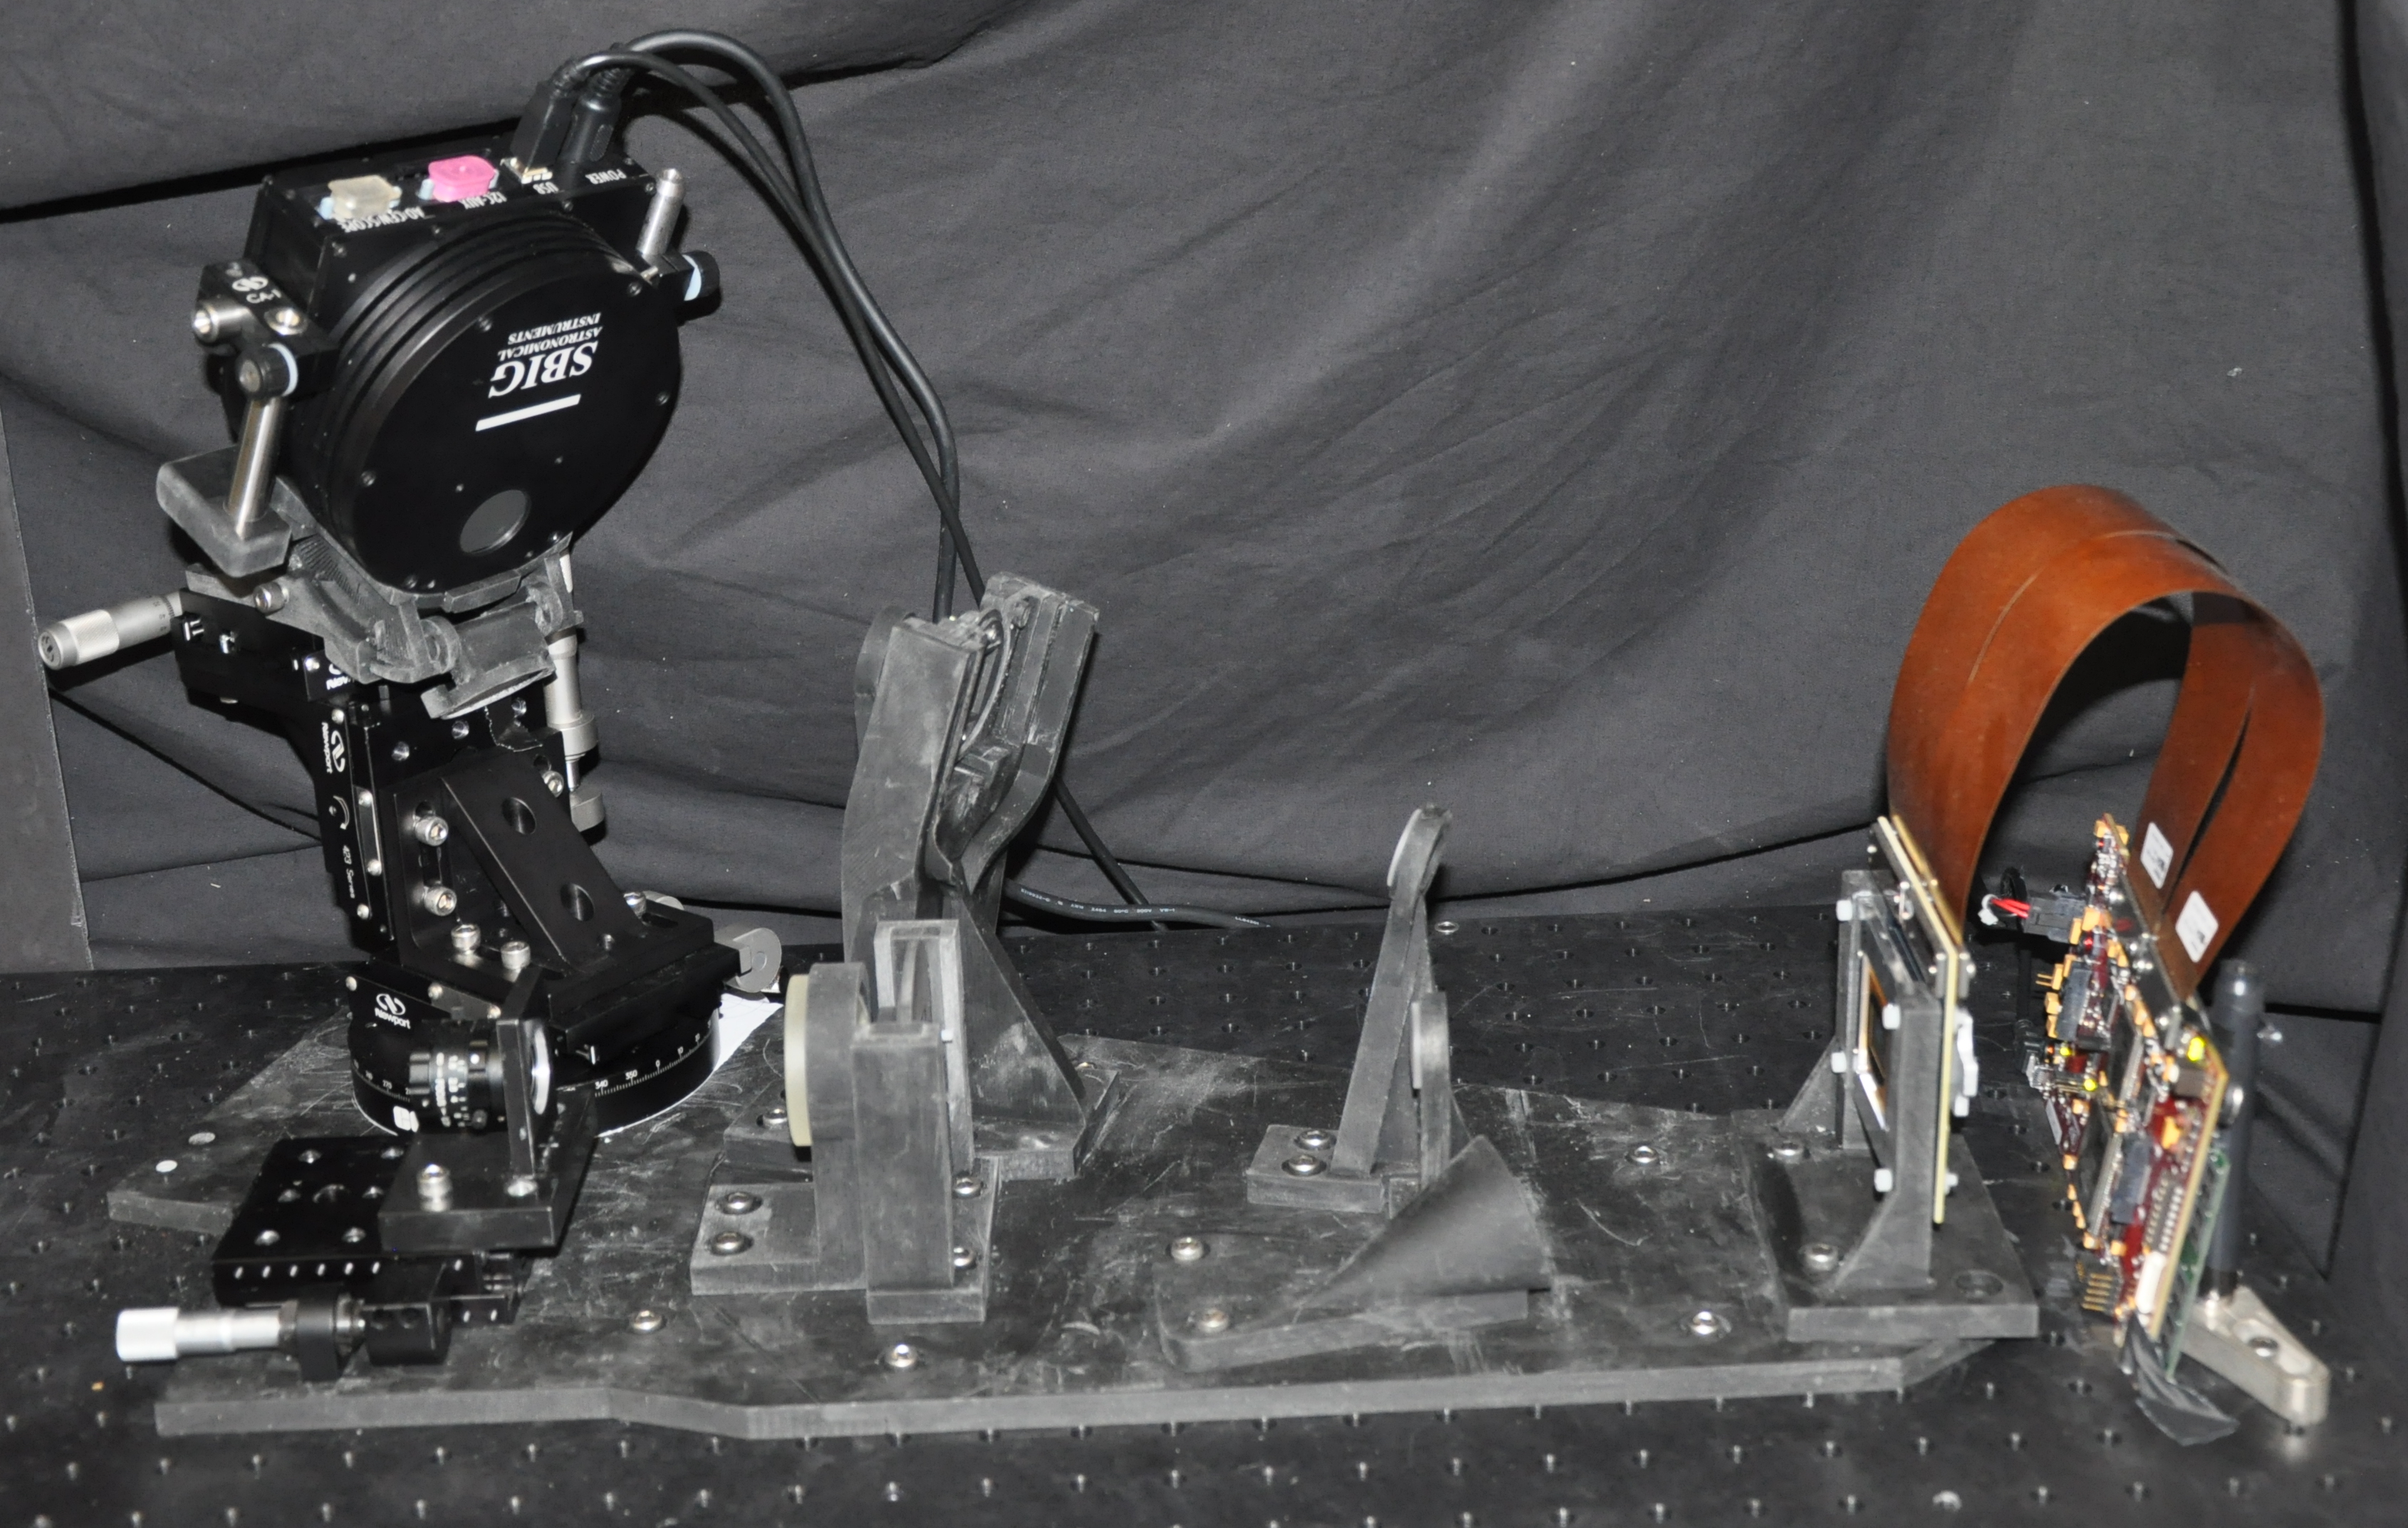
\includegraphics[height=3.7in]{afssicPhoto1.JPG}\\
	\captionof{figure}[Photograph of AFSSI-C.]{Photo of \gls{afssi-c}}
	\label{fig:afssicPhoto1}
\end{figure}

For a repeatable, programmable synthetic datacube source, we used an LED display (Dell P2311H LED monitor with 248 \textmu m pixel pitch). Though this limits the spectra we were able to generate, it still allows for programmable spectra at every spatial location. The center 1080 $\times$ 1080 pixels are used to generate the source spectral datacubes. Spectra consist of combinations of the RGB monitor colors.

The \gls{afssi-c} operated at a spectral range of 425-625 nm, which is approximately the visible wavelength range. We placed thin-film spectral filters in the collimated space to attenuate light outside of this range. The system is designed for $N_{\lambda} = 38$ spectral channels, resulting in roughly $5$ nm/spectral channel. The system magnification to the \gls{dmd}, which then dictates the lateral spread allowed per spectral channel, requires custom 0.10 lines \textmu m holographic blaze gratings as the dispersive elements, fabricated by Wasatch Photonics. The gratings are designed to minimize diffraction in all the orders except the first order. 

The \gls{dmd} used in our experimental prototype was manufactured by Texas Instruments, it is a DLP Discovery 4100 \gls{dmd} development kit, with the DLP9500 0.95" 1080p \gls{dmd} chipset. The \gls{dmd} has 1080 $\times$ 1920 10.8 \textmu m mirrors on the array, and the mirrors pivot 12 degrees on a diagonal axis. The \gls{dmd} is oriented such that the bottom of the array is parallel to the optical table, which forces the second arm of the \gls{afssi-c} to rise off the optical table at an angle of 17.5 degrees; this orientation was chosen so that the mirrors would be oriented as squares rather than diamonds. While the periodic structure of the \gls{dmd} can produce strong diffraction for certain types of illumination, no diffraction effects are observed in the \gls{afssi-c} as the light incident on the \gls{dmd} is incoherent. 

A Santa Barbara Instrument Group (SBIG) ST-10XME detector with a 2184 $\times$ 1472, 6.8  \textmu m pitch \gls{ccd} as the camera. Due to the angle of the optical axis of the second arm of the \gls{afssi-c}, a goniometer was constructed using a rapid prototyping 3D printer to facilitate easy alignment of the SBIG camera \cite{dunlop-gray2015phdthesis}.

%ecause we are interested in a quantitative system analysis, we compare measurements on the discretized detector to what was projected by our discretized source. The layout dimensions, component pixel size, and lens design were tuned to yield pixel groups---referred to here as \gls{sp}s---at each component that are an integer number of the component pixel, or in the case of the \gls{dmd}, integer number of mirrors. We therefore have the following \gls{sp} dimensions: $16 \times 16$ pixels on the source, $8 \times 8$ \gls{dmd} mirrors, and $12 \times 12$ pixels at the detector.

Once the optical layout was finalized, the physical system was designed in SolidWorks. The lens mounts, detector mount, \gls{dmd} mount, beam dump, and locating plates were then fabricated on a Eden 350 rapid prototyping 3D printer.

Light baffling is utilized to shield the system from ambient light as well as stray light within the system. A baffling structure was designed and printed to surround the detector, with smaller baffling elements to attenuate stray light around the optical paths.


\subsection{Implementing Codes}

One of the practical considerations of the coding scheme in the \gls{afssi-c} is that the pPCA algorithm generates both positive and negative elements in the feature vectors. These are analogous to having positive and negative weights in the weighing problem. Unfortunately, with incoherent light, one is unable to make simultaneous positive and negative measurements because we cannot easily manipulate the phase of the electric field. Therefore, in the \gls{afssi-c} we are forced to take two camera exposures for each measurement step and subtract the negative set of measurements from the positive set of measurements. This means that an additional noise term is added to each measurement step. For the rest of this chapter, when I say measurement or measurement step, I really mean one  measurement step which records two camera exposures.

Another practical issue is that the \gls{dmd} we used only allows a binary mode of operation. Either the mirror reflected the light towards the second arm or it reflected light towards the beam dump. In practice any positive element is set to $1$ and any negative element is set to $-1$. 

\subsection{Calibration}

One reoccurring topic in this dissertation is calibration. In computational sensing the measurement may not look anything like the signal-of-interest. Just like in the \acrfull{scout}, the \gls{afssi-c} relies heavily on several calibration procedures which involves spatial, spectral, and noise measurements for optimal classification performance.


\subsubsection{Spatial Calibration}

One of the major opto-mechanical issues in the \gls{afssi-c} is caused by the geometry of the \gls{dmd} with respect to the second arm. The \gls{dmd} plane is normal to the optical axis of the first arm, but it is at an angle (equal to twice the tilt of the mirrors on the diagonal) to the second arm. One can think of the \gls{dmd} plane as the object plane for the second arm of the system. Since the \gls{dmd} is tilted, this creates an Scheimpflug distortion: a tilted object plane images to tilted image plane \cite{smith1966modern}. 

Because of Scheimpflug distortion, the image of the monitor physical pixels are not aligned to the rectangular grid of pixels on the \gls{fpa}, see \Cref{fig:rawDetReadoutOfUofALogo}. Even worse there is not a one-to-one relationship of \gls{fpa} pixels to object scene pixels since the magnification is not constant over the \gls{fov}.  In order to produce optimal performance we need to know the mapping of monitor to \gls{fpa} pixel locations. The goal of spatial calibration is to make a set of measurements in which we can infer a parameterized relationship from \gls{fpa} physical pixel coordinates to monitor physical pixel coordinates. 


\begin{figure}[htb]
	\centering
	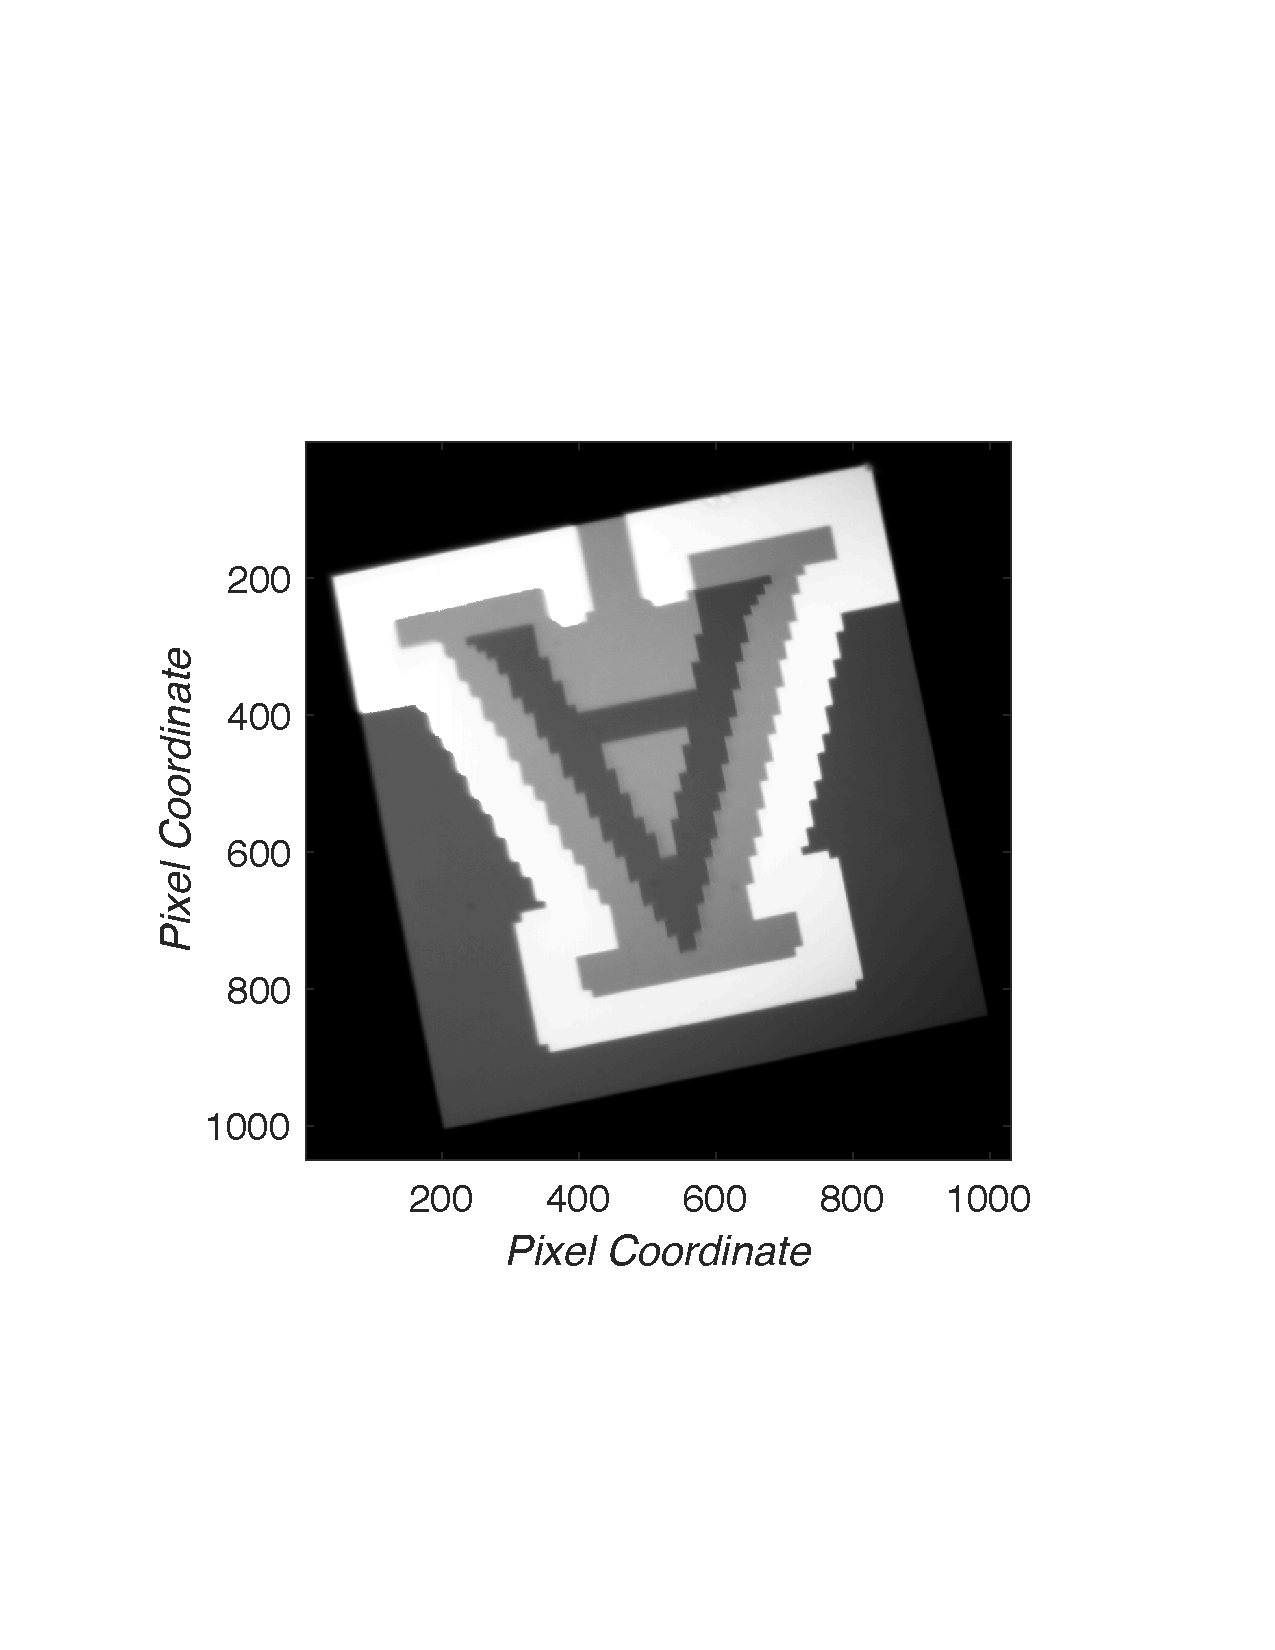
\includegraphics[scale=0.75]{rawDetReadoutOfUofALogo}\\
	\captionof{figure}[The image produced by the camera without any post-processing.]{The image produced by the camera without any post-processing.}
	\label{fig:rawDetReadoutOfUofALogo}
\end{figure}


Due to spatial resolution constraints and other practical issues, we grouped several physical pixels together in a \acrfull{sp}. For example, in our experiment we have an effective resolution of 64 $\times$ 64 \gls{sp}s. However, on the monitor a \gls{sp} actually consists of 16 $\times$ 16 physical pixels on the source. Similarly, on the \gls{dmd} a \gls{sp} consists of 8 $\times$ 8 physical pixels (mirrors) and on the detector a \gls{sp} consists of 12 $\times$ 12 physical pixels.


A straightforward approach to inferring the relationship between \gls{fpa} and object scene pixels would be to energize each physical pixel on the \gls{roi} one at a time and record the image on at the physical pixel. We could then create a look-up table for each \gls{fpa} pixel to infer where from the LED this came from. However, energizing each of the 1024 $\times$ 1024 physical pixels at 5 seconds per exposure will take approximately 61 days. We are therefore forced to infer the spatial transform from a small number of physical pixels images.

At this point we are only concerned with how the the LED monitors appear on the \gls{fpa} image. The alignment of the \gls{dmd} does affect the image quality and location, but the pattern of the \gls{dmd} only affects the radiance of an image point. Therefore, we set the entire \gls{dmd} mirror pattern to reflect towards the second arm. In this state, the \gls{dmd} acts like a normal mirror. 

First the monitor displays a grid of white dots, \Cref{fig:gridOfWhiteDotsForSpatialCalibration1}. The number of dots can be then be increased for better accuracy but increases the calibration time. The list of monitor physical pixel coordinates where the center of each dot appeared on the monitor is then saved.

\begin{figure}[htb]
	\centering
	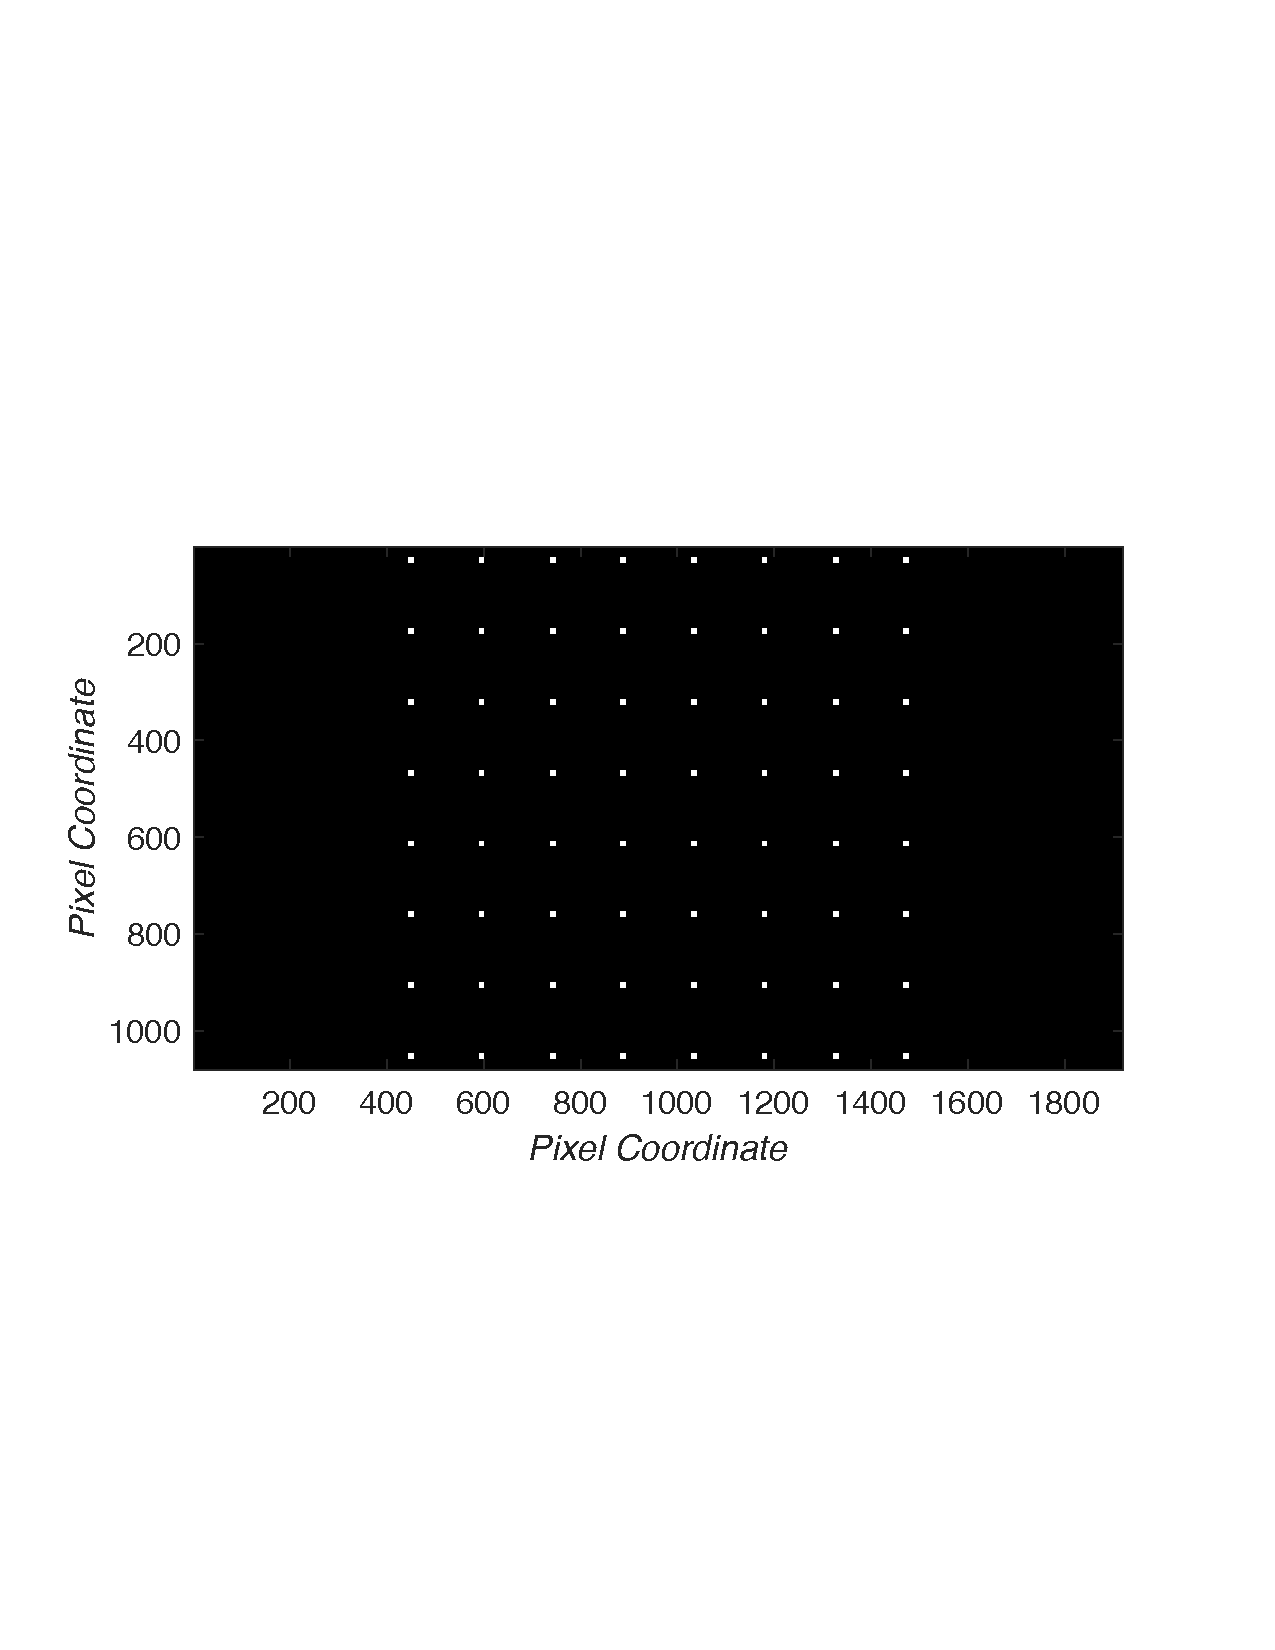
\includegraphics[scale=0.81]{gridOfWhiteDotsForSpatialCalibration1}\\
	\captionof{figure}[Spatial Calibration Grid of Dots Used In \gls{afssi-c} Experiment]{An array of white dots is displayed on the monitor as part of the spatial calibration. The image of this grid is recorded, the centroids are estimated and a spatial transform is inferred between the physical pixel coordinates of the LED monitor and the \gls{fpa}}
	\label{fig:gridOfWhiteDotsForSpatialCalibration1}
\end{figure}

A raw camera image is captured and stored, see \Cref{fig:detReadOutOfDots}. To account for hot pixels and systematic error in the system the camera image of the all black monitor is subtracted from the camera image of the array of white dots which gives us the dark subtracted image of white dots. The dark subtracted detector image is then thresholded to prevent noisey pixels from being counted as one of the images of the white dots from the monitor. All values above the threshold is set to 1 while all values below the threshold is set to 0.

Using a built-in MATLAB \texttt{regionprops} function with the optional \texttt{centroid} argument, we can infer the center pixel, centriod, for each of the white dot images in the thresholded image. This function generates a list of pixel coordinates from the thresholded image. Each pixel coordinate is associated with the center of each white dot in the image. Often times however, we get a list of coordinates is that more or less than the number of white dots displayed onto the monitor. At this point, we may need to change the threshold value to return the same number of coordinate pairs as dots displayed on the monitor. For example if we have an 8 $\times$ 8 grid of dots we expect a list of 64 detector pixel coordinate pairs. As a sanity check, we can create an image of the where the inferred centriods are and overlay it on thresholded image of the grid of white dots. The image of the centriods should be approximately on top of the image of each white dot, see \Cref{fig:centriodsOverlayedOnTheThresholdedImage}.

\begin{figure}[h]
\includegraphics[scale=0.7]{detReadOutOfDots}
\centering
\caption{The detector image of the array of white dots as part of the spatial calibration}
\label{fig:detReadOutOfDots}
\end{figure}

\begin{figure}[h]
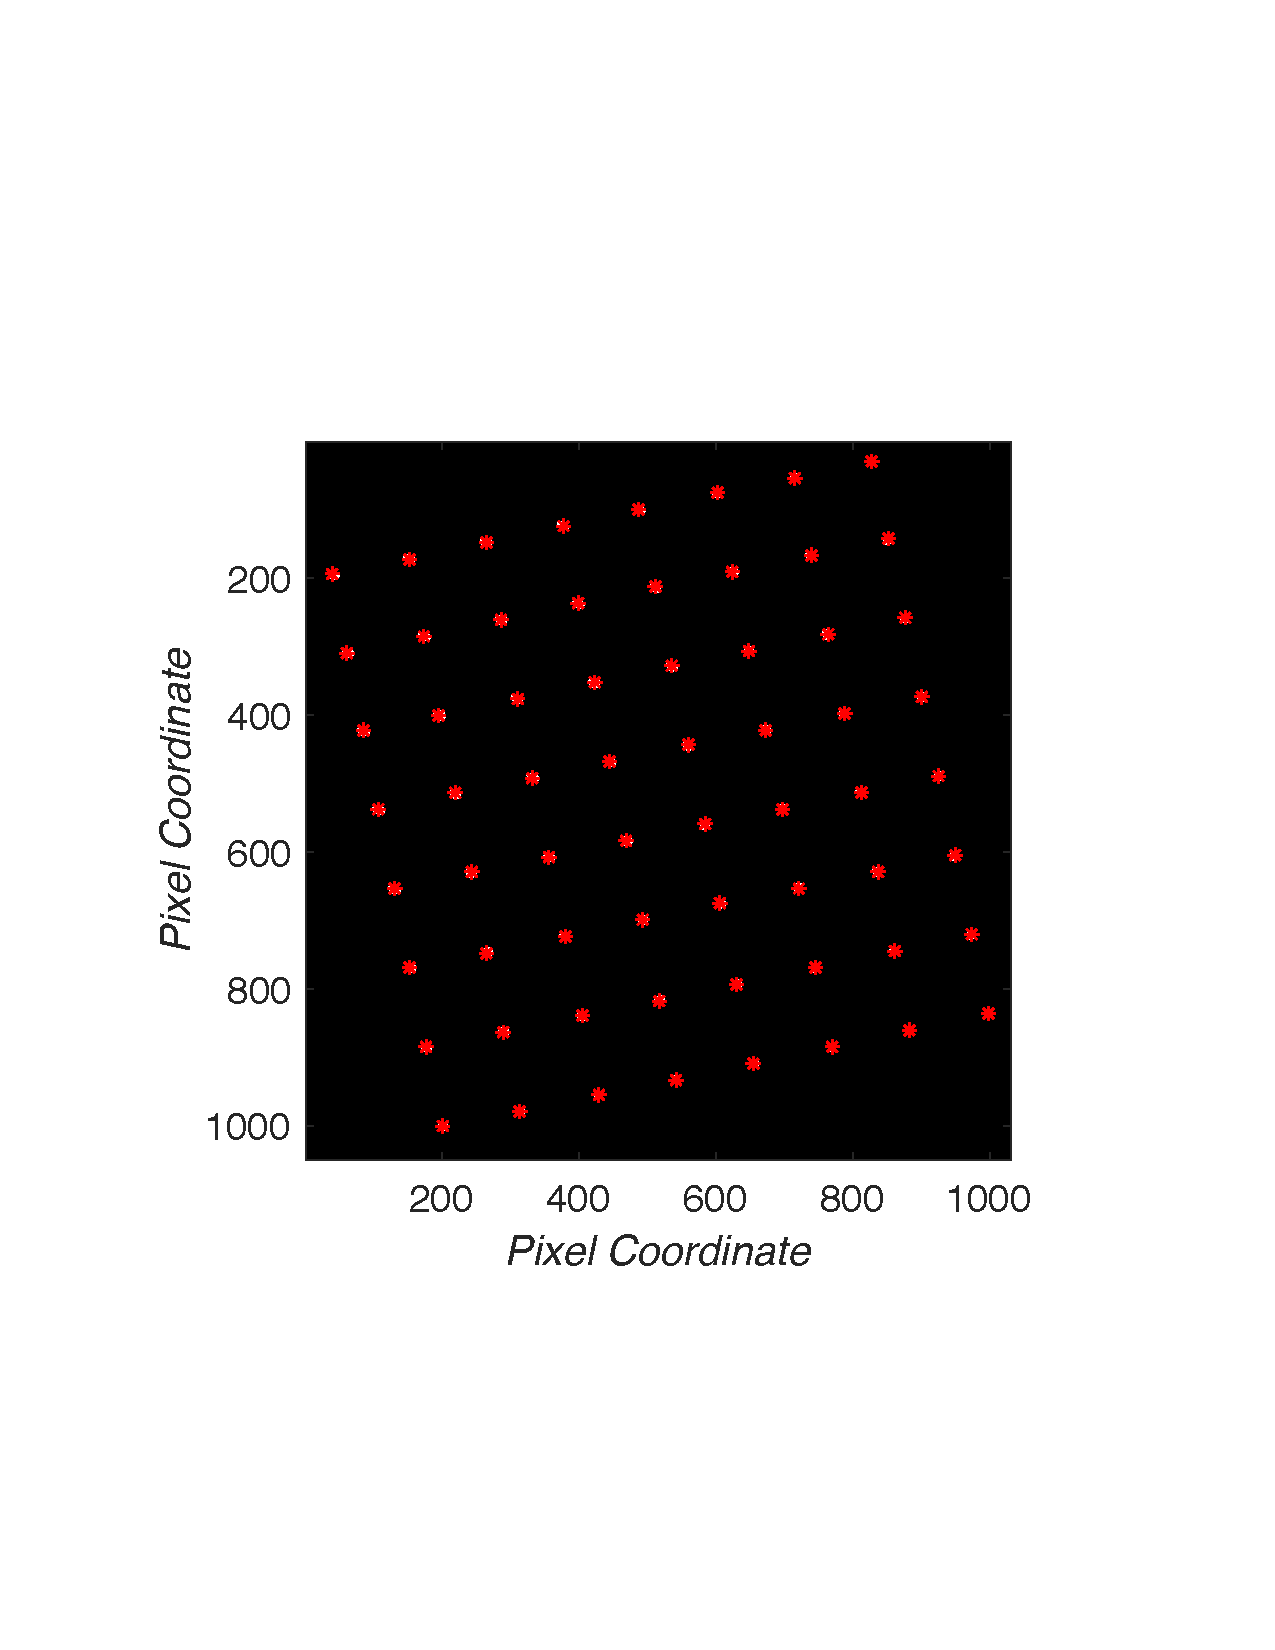
\includegraphics[scale=0.7]{centriodsOverlayedOnTheThresholdedImage}
\centering
\caption{The detector image of the array of white dots as part of the spatial calibration}
\label{fig:centriodsOverlayedOnTheThresholdedImage}
\end{figure}

Each dot is added to the monitor scene one at a time to prevent accidently associating the wrong dot on the image. Doing this each time the \gls{afssi-c} is calibrated is time consuming, since we need at least as many \gls{fpa} exposures as there are dots in the object scene. In practice, we use MATLAB to look up the locations from the last spatial calibration and if we believe the instrument has not been misaligned since then, we look in a neighborhood of pixels around the last dot locations and compute the centroids of the dots, see \Cref{fig:theFinalSquareLocatesTheFinalDot}.


\begin{figure}[h]
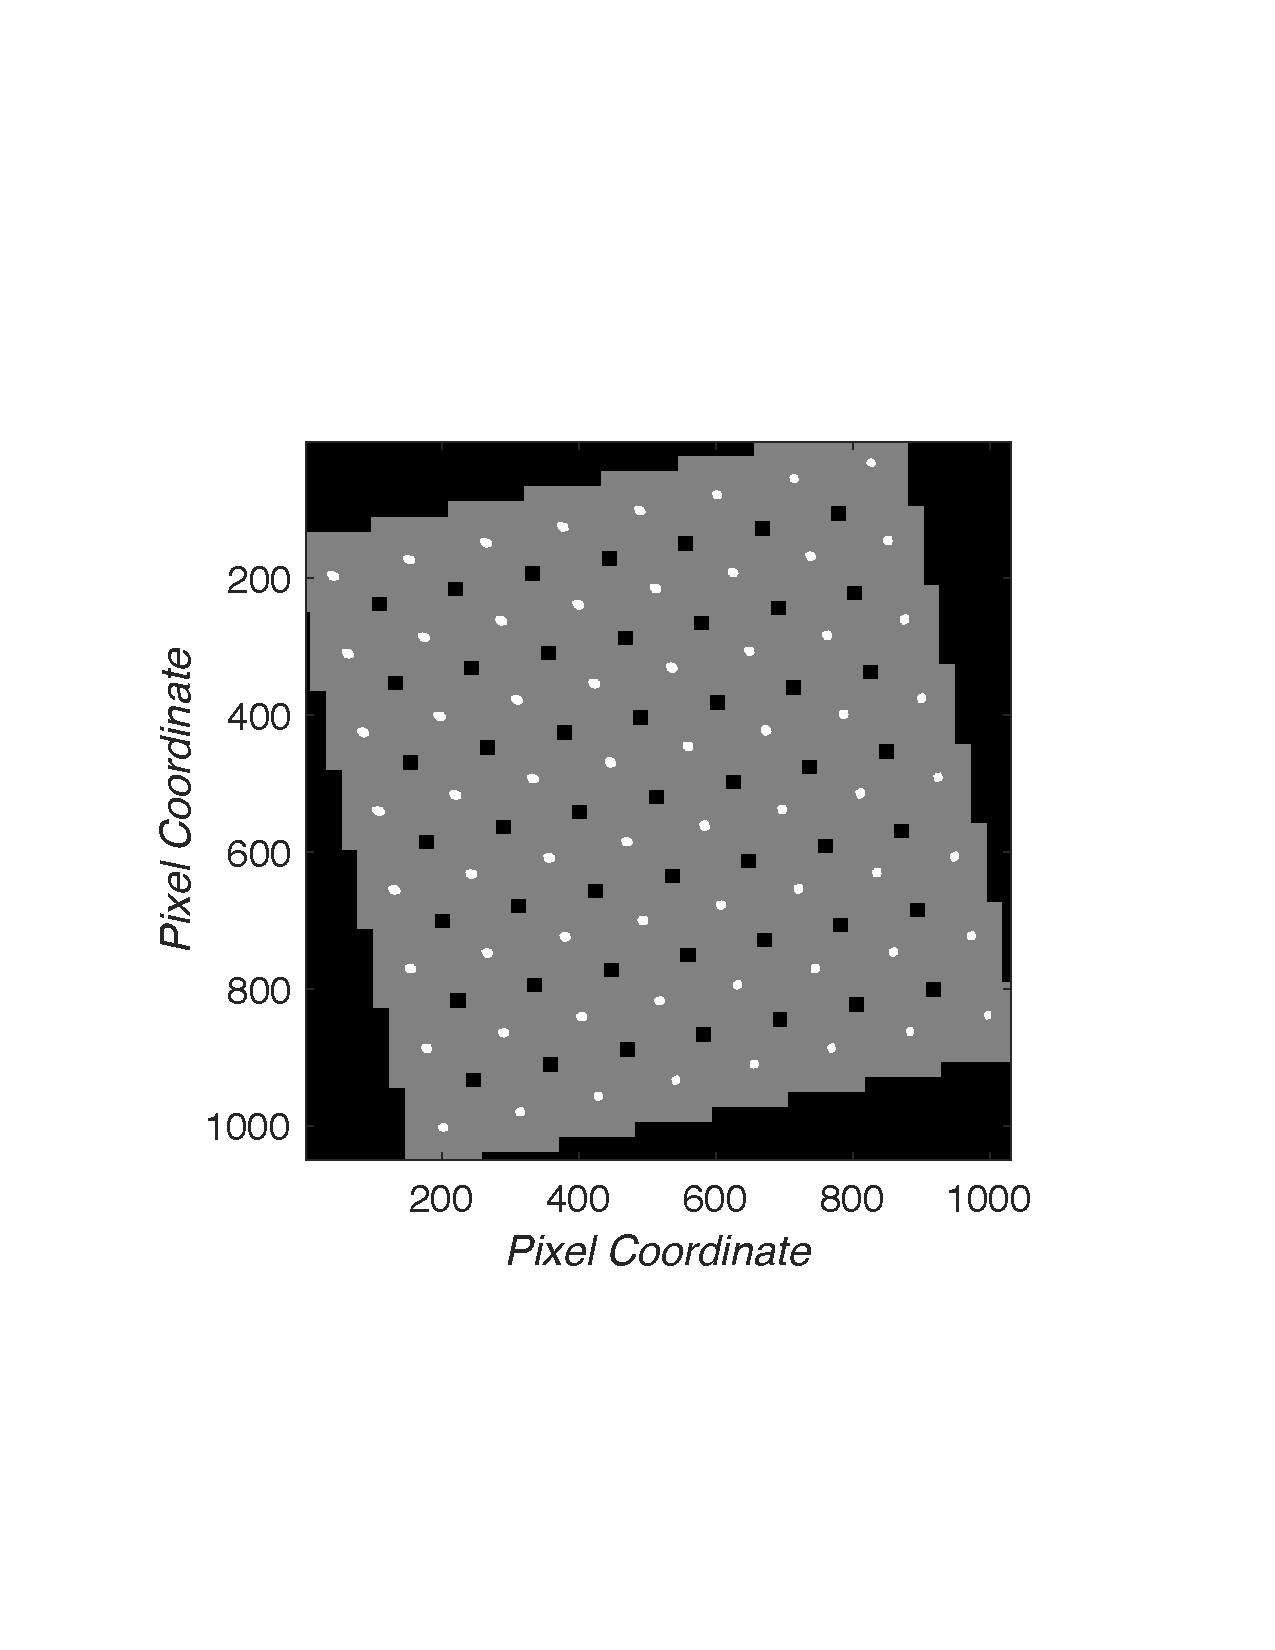
\includegraphics[scale=0.7]{theFinalSquareLocatesTheFinalDot}
\centering
\captionof{figure}[Speeding Up Spatial Calibration By Looking In Regions Around Previous Spatial Calibration Image Dots]{Instead of displaying the dots one at a time, we use the location of the dot images from the last spatial calibration and search in a rectangular region around those coordinates for the new dots. This greatly speeds up the spatial calibration since each exposure is approximately 3-5 seconds.}
\label{fig:theFinalSquareLocatesTheFinalDot}
\end{figure}


Now that we have a list of dot centers in the monitor pixel coordinates and a list of dot centers in the detector pixel coordinates, we use the MATLAB function \texttt{cp2tform}, which takes the list of control points and uses them to infer the spatial transform. This transform is a parameterized relationship between every single physical pixel coordinate on the monitor and physical pixel coordinate on the detector. 

Each \gls{sp} contains $16 \times 16$ physical pixels, using the spatial transform, we known which detector pixels these physical pixels will image to. The average value of all the physical pixels from the \gls{fpa} image correspond to the \gls{sp} value. Thus we can reverse the effects for any image rotation or translation at the \gls{fpa} plane.

As part of the calibration procedure, an image is saved by turning on the entire DMD and measuring the intensity at each spatial location with the monitor set to white at full intensity. One can think of this image as an intensity map, providing information as to which locations have more throughput than others in the \gls{fov}. During the classification operation, each camera image is normalized by this intensity map, while the spectral library at each location is normalized by the integration of the white spectrum (which has the system spectral response information folded into it), allowing the classification decisions to be made. 


\subsubsection{Spectral Calibration}

Unfortunately, due to vignetting and imperfections in the gratings the spectral response of the \gls{afssi-c}, the combined optical system produces a shift-invariant spectral response. To correct for this we developed a calibration procedure to measure how the spectral response of the optical system varies over the region-of-interest in the \gls{fov}. 

A flowchart of the spectral calibration is shown in \Cref{fig:grabRawDetectorImagesForResponseCubes}. Remember that in the \gls{afssi-c} architecture, the first column of mirrors on the \gls{dmd} reflects light corresponding to the first spectral channel of the first spatial column. The second column of mirrors reflects light corresponding to the first spectral channel of the second spatial column and also reflects the light in spectral channel 2 of the first spatial column, and so on, see \Cref{fig:fastSpectralCalibration}. Also, the dual-disperser architecture of the \gls{afssi-c} means that light from a single spatial pixel images to a single spatial pixel on the \gls{fpa}, regardless on what pattern is being displayed on the \gls{dmd}. In other words, in a single camera image image we can measure the intensity of different spectral channels of adjacent spatial locations along a row by turning on only one \gls{dmd} mirror. Therefore, we can turn on an entire row of pixels in the monitor and realize that different \gls{fpa} images correspond to different spectral channels for each spatial location. 

Also remember that the dispersion is only in the horizontal direction, along the columns of the \gls{dmd}. Therefore, we can set the entire \gls{roi} to display the same spectrum. Then sweep the entire column of the \gls{dmd}. In our experiment, the number of effective \gls{dmd} \gls{sp} columns is equal to the number of monitor \gls{sp} in a row plus the number of spectral channels minus one 
%
\begin{equation}
	N_{d_x} = R_x + N_{\lambda} - 1
\end{equation}
%
Therefore, we had 101 \gls{dmd} \gls{sp} columns. So the first 38 camera images corresponds to the 38 spectral channels in the first spatial \gls{sp} column. Then images 2 to 39 correspond to the first 38 spectral channels in the second spatial \gls{sp} column. 

Another way to reduce the spectral calibration time is by realizing that we can turn on two \gls{dmd} \gls{sp} columns at a time. This is because we only have 38 spectral channels and 101 DMD \gls{sp} columns. So in our calibraiton procedure we turn on two \gls{dmd} \gls{sp} columns at a time each 50 \gls{sp} columns apart. Then for each spectrum in spectral library we only need 51 exposures. If we assume a 5 second expsoure this only takes about 20 minutes. In practice we use a much longer exposure time to increase the \gls{snr} of each \gls{fpa} exposure. The total time for a four class spectral library is approximately 4 hours.


\begin{figure}[h]
	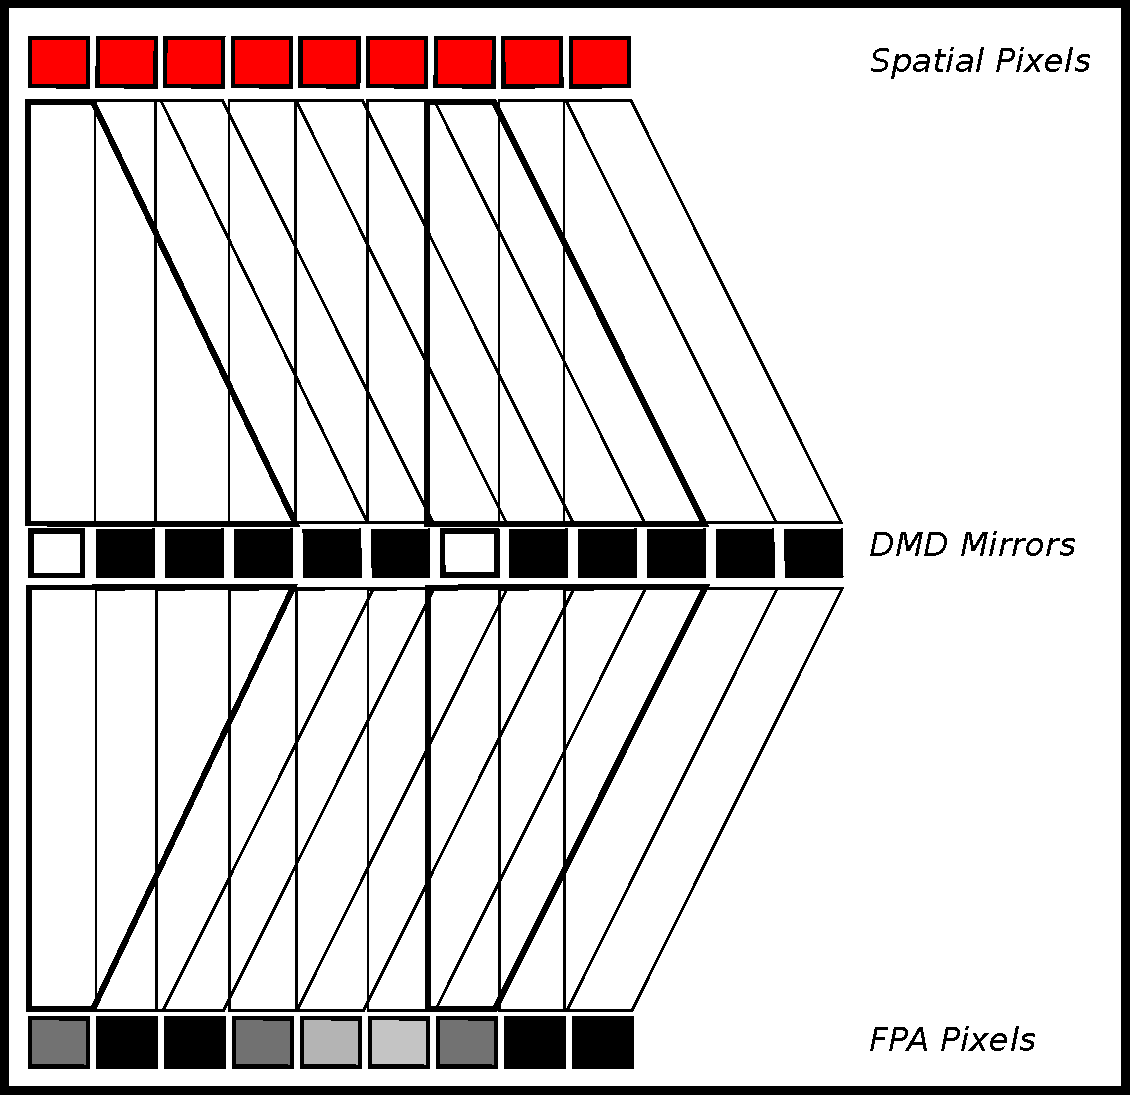
\includegraphics[scale=0.7]{fastSpectralCalibration}
	\centering
	\captionof{figure}[Depiction of spectral calibration]{In order to speed up the spectral calibration we turn the entire monitor ROI to the same spectrum and sweep two DMD columns at a time.}
	\label{fig:fastSpectralCalibration}
\end{figure}

\clearpage
	\begin{figure}[H]
	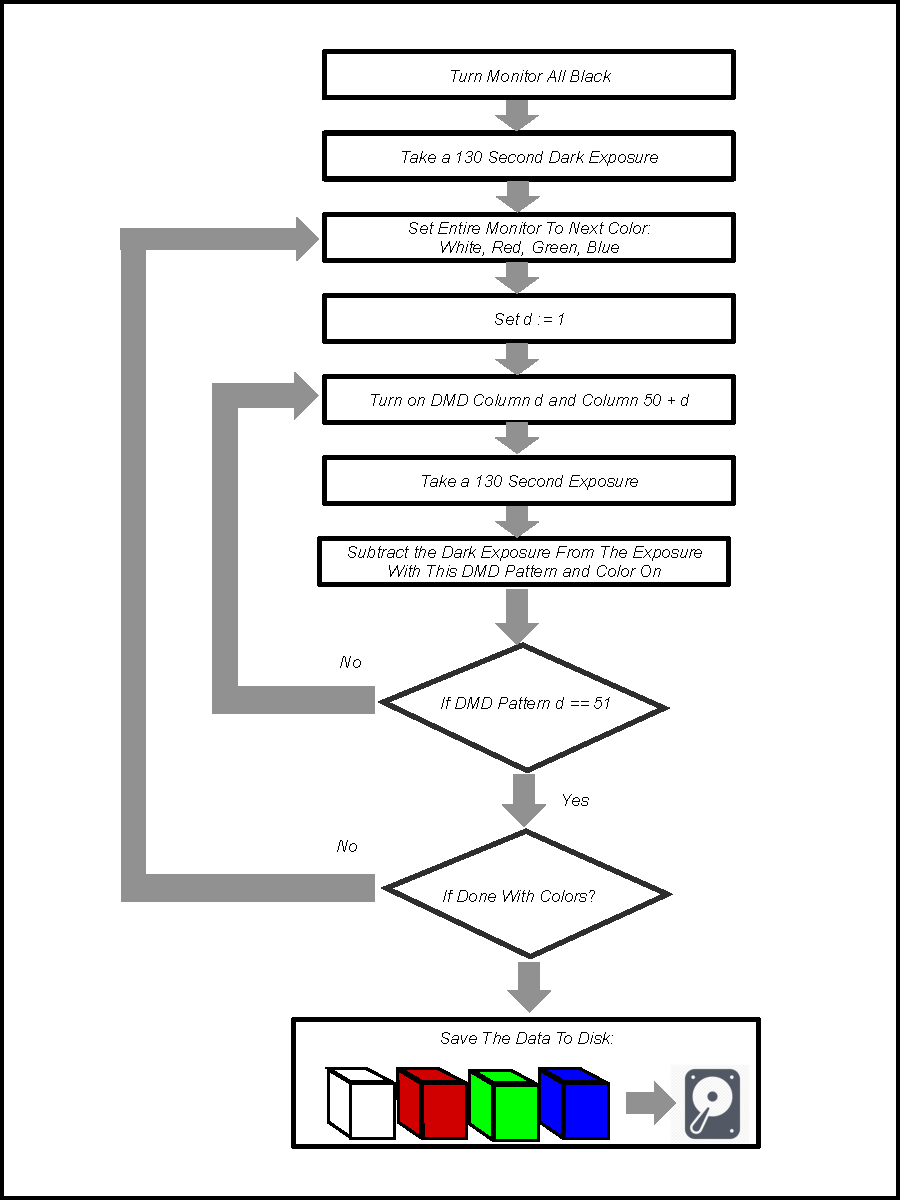
\includegraphics[scale=1.0]{grabRawDetectorImagesForResponseCubes}
	\centering
	\captionof{figure}[Depiction of spectral calibration]{In order to speed up the spectral calibration we turn the entire monitor ROI to the same spectrum and sweet two DMD columns at a time.}
	\label{fig:grabRawDetectorImagesForResponseCubes}
\end{figure}


\subsubsection{Noise Model Calibration}

As I discussed in \Cref{ssec:updatingProbabilities}, the adaptive algorithm we used to make classification decisions compares the ratio of posterior probabilities by updating ratios of the likelihoods after each measurement. The likelihood is defined as the probability of the measurement given that the hypothesis is true. This probability is given by the noise model using \Cref{eq:noiseModel1}. Accurate estimation of the noise standard deviation, $\hat{\sigma}$, is required for optimal classification rates. 

If $\hat{\sigma}$ is much larger than the actual value,  $\sigma$, then the probability for different spectral classes will tend to be similar. However, as I discussed, the \gls{ppca} algorithm depends on weighting the probability of some classes higher than others to outperform non-adaptive systems. This may lead to longer convergence times to the correct class. If the $\sigma$ is too small then the algorithm may converge to the wrong class. 

Fortunately estimating the noise of the system is a relatively straightforward. At each spatial \gls{sp} location we randomly choose one the spectra from the spectral library and display it, then the we display a random pattern on the entire \gls{dmd} record the camera image and compare the measured intensity value at each spatial location to what we expected from the simulated camera image. This is repeated several times until we have sufficient statistics to plot the distribution of the differences between measured and expected intensities, see \Cref{fig:noiseCalFit}. Using the MATLAB \texttt{fit} function with the one-dimensional Gaussian option \texttt{gauss1},we fit a Gaussian to the data to estimate the standard deviation of the noise, $\hat{\sigma}$.

The value of $\sigma$ is the intrinsic amount of noise in the instrument. It takes into account all possible sources of noise in the \gls{afssi-c}. However, we would like to vary the total amount of noise to see how the experimental classification performs compared to simulation and how the it performs compared to various other imaging spectrometers. This is done in post-processing by adding normally distributed noise with standard deviation $\sigma_{added}$ to the measurements. Since the intrinsic system noise is approximately Gaussian, the total variance is thus

\begin{equation}
	\sigma_{total}^2 = \sigma^2 + \sigma_{added}^2
\end{equation}

\begin{figure}[h]
	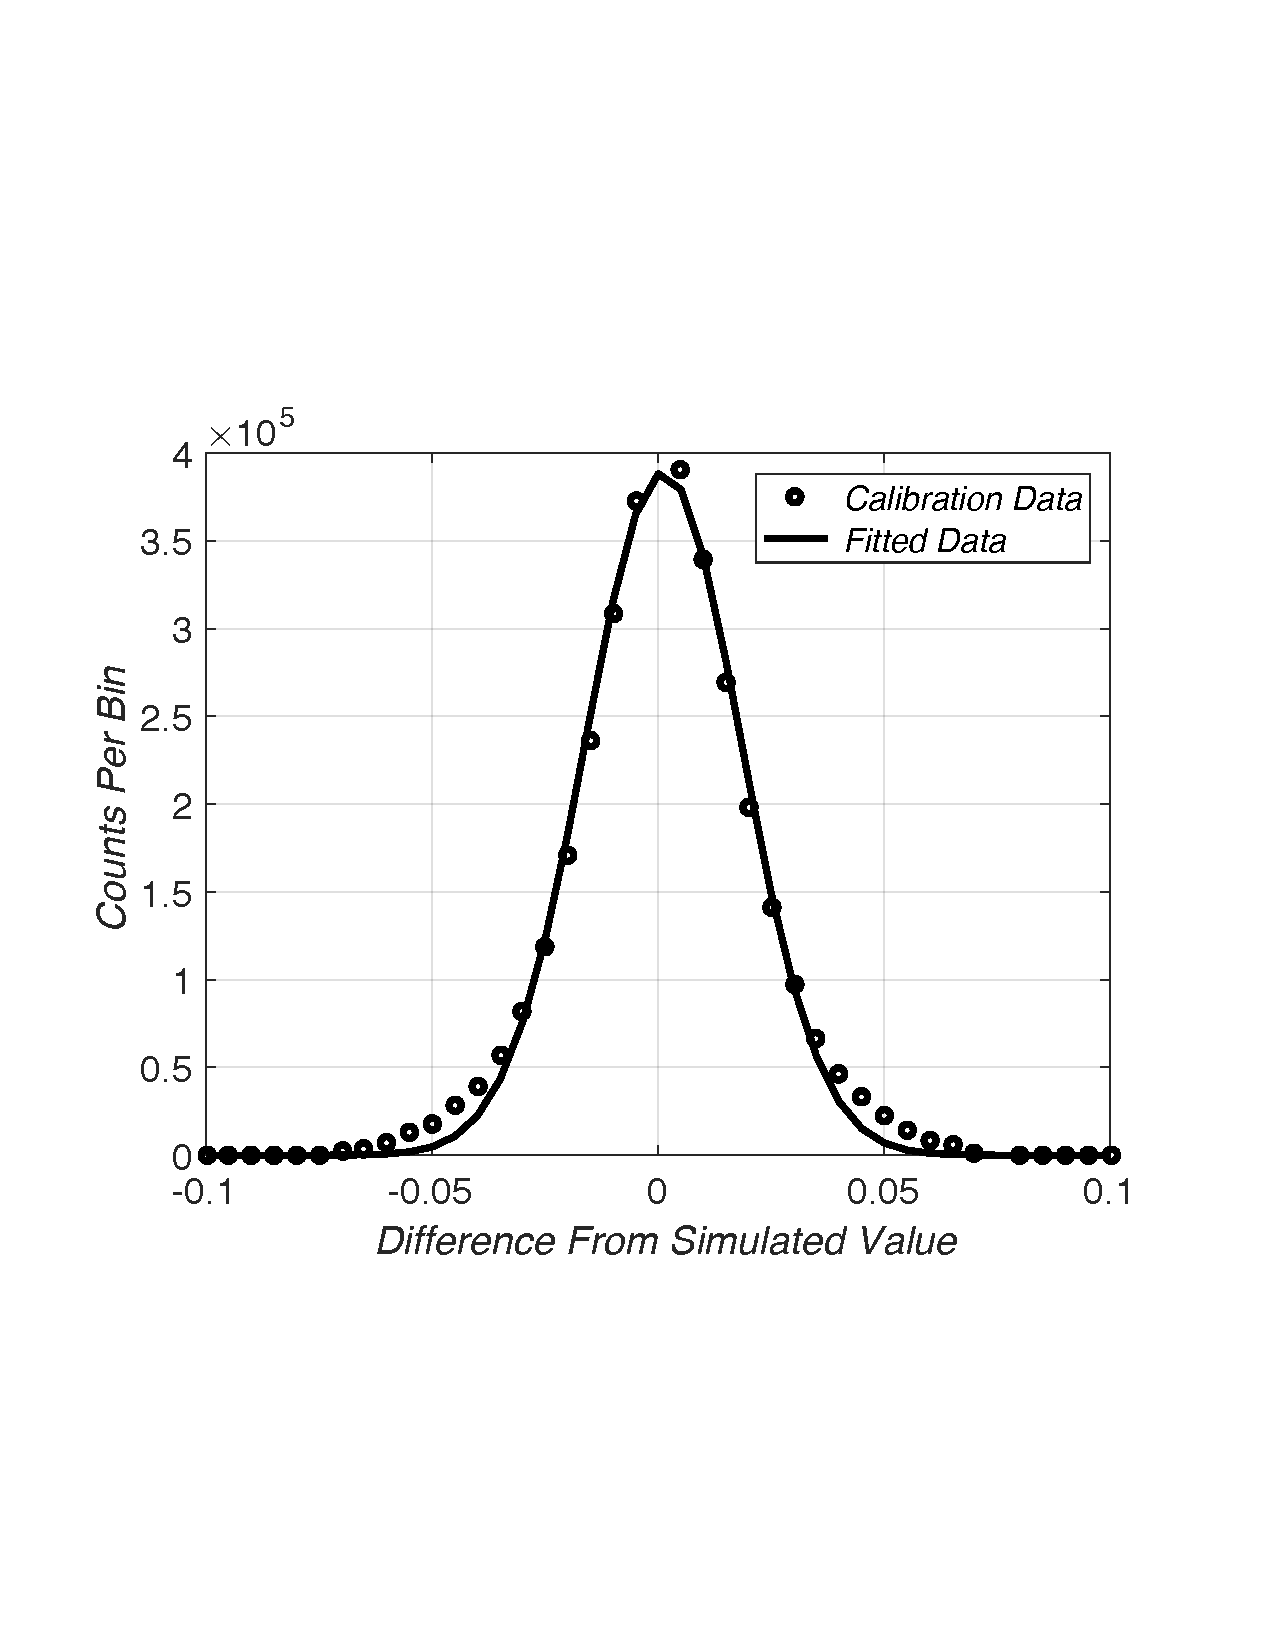
\includegraphics[scale=0.8]{noiseCalFit}
	\centering
	\captionof{figure}[Estimating the System Noise]{Estimating the System Noise: The circles represent the distribution of difference between the measurement and expected values of randomly chosen spectra with random spectral filters. The solid line represents a Gaussian fit, which allows us to estimate the standard deviation of the system noise.}
	\label{fig:noiseCalFit}
\end{figure}

\section{Experimental Results}


\Cref{fig:afssicExpResults3InChap} presents experimental classification results at 0, -3, and -6 dB TSNR after measurements. Measurements 1 through 30 are presented in Appendix \ref{app:afssicExpResults}. As the classification difficulty increases (lower TSNR), the adaptive algorithm takes more measurement steps to correctly classify. 

 \begin{figure}[htb]
  \centering
  % Requires \usepackage{graphicx}
  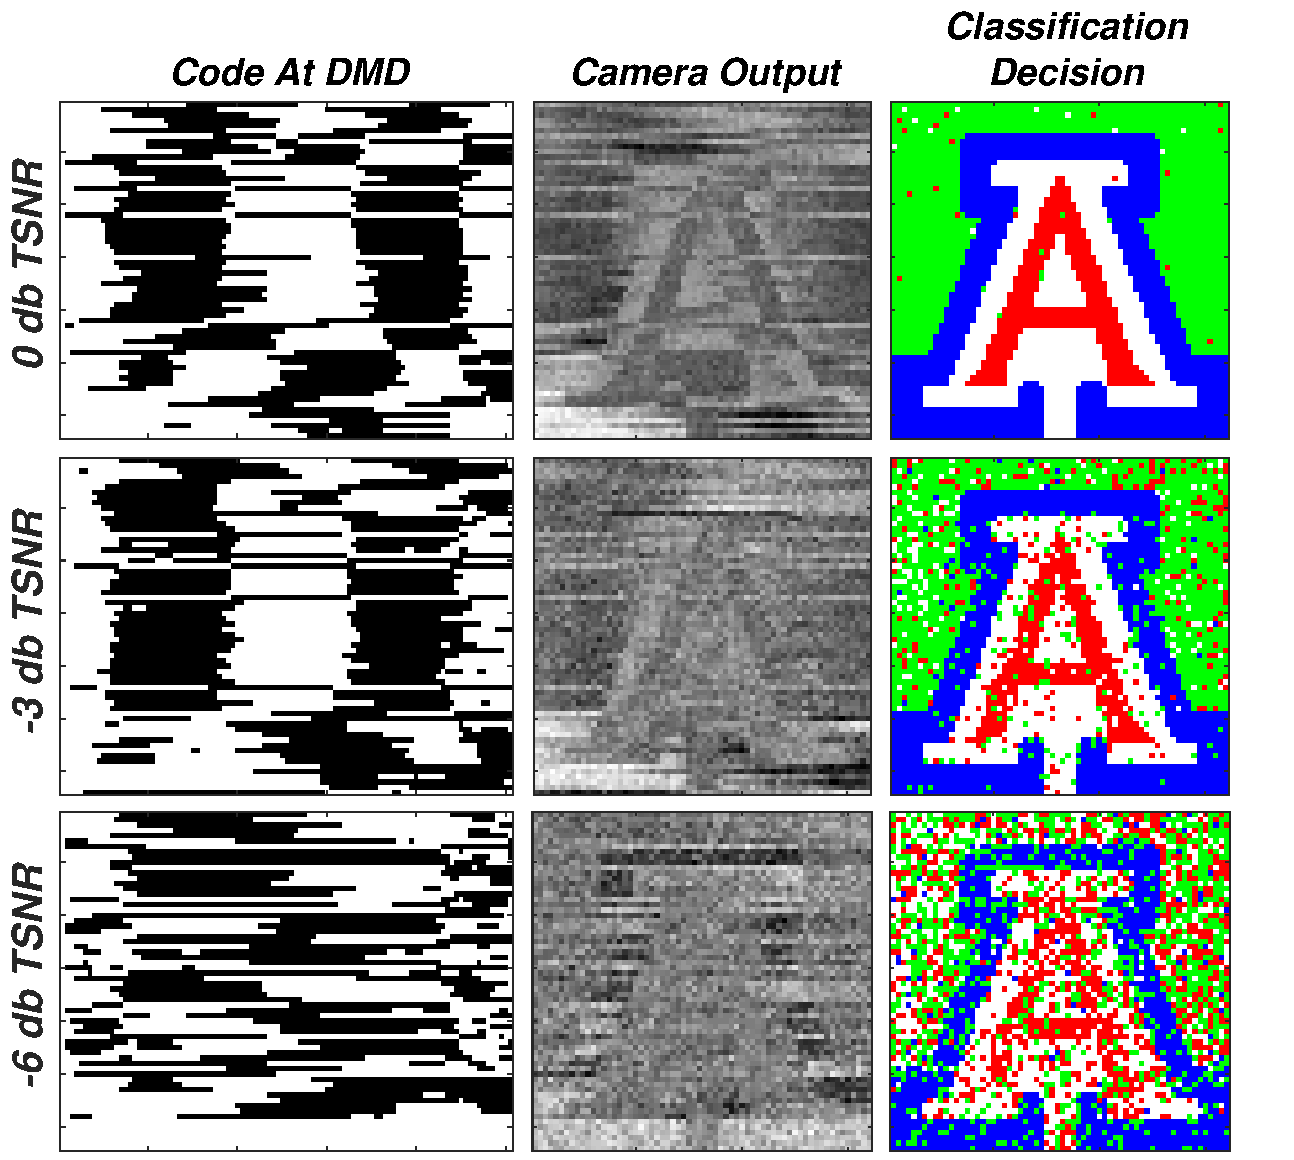
\includegraphics[scale=0.72]{afssicExpResults3}\\
  \caption{Data from after the third measurement step at 0, -3, and -6 dB TSNR. The left column is a depiction of the \gls{dmd} code, center is the output from the detector, and the right is the classification decision at the current measurement.}\label{fig:afssicExpResults3InChap}
\end{figure}

The experimental classification rates that we obtained agree well with simulation. \Cref{fig:SIMmultiTSNR} shows the performance of the \gls{afssi-c} experimental results and the simulated values. The simulated and experimental data are the average of 30 simulations and 10 experiments, for each of the four \gls{tsnr} values representing several levels of increasing classification difficulty (0, -3, -6, and -9dB TSNR).
%
%Experimental data with simulation
\begin{figure}[htb]
 	\centering
  	% Requires \usepackage{graphicx}
  	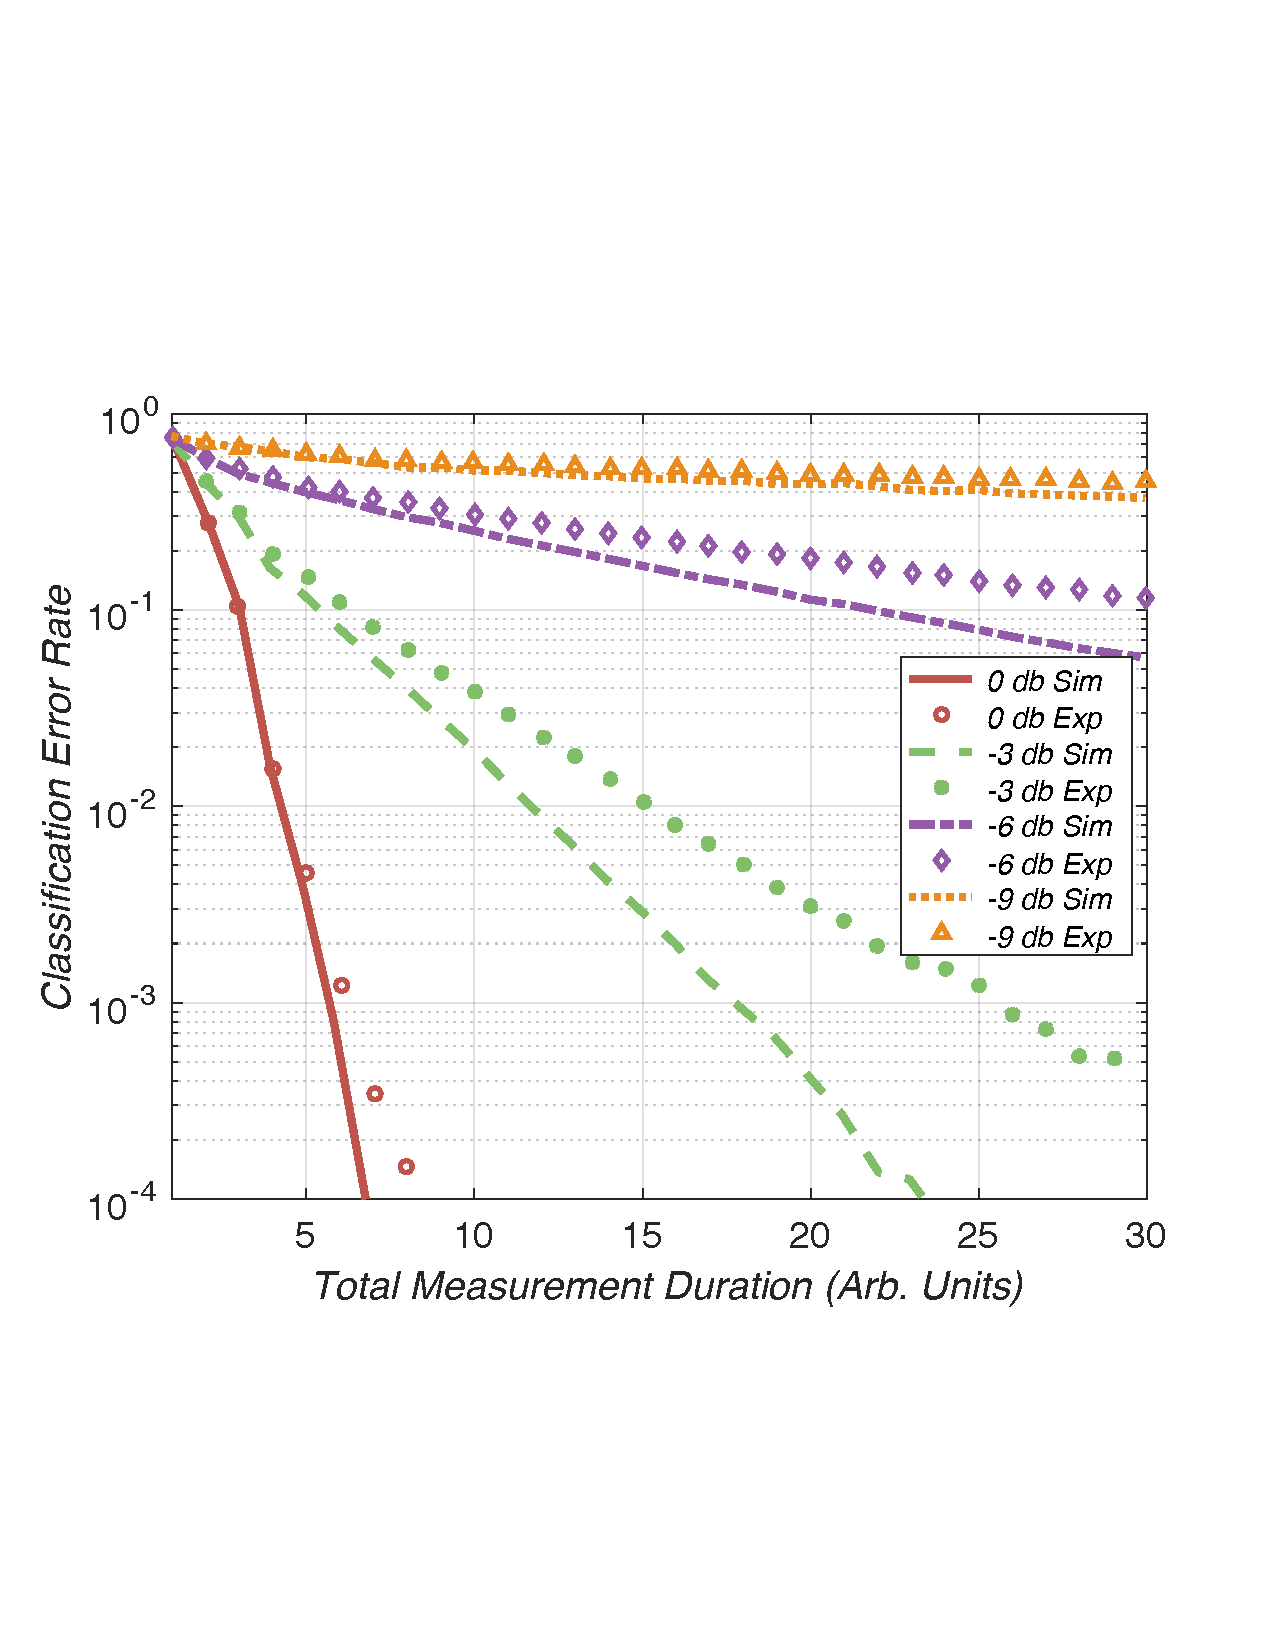
\includegraphics[scale=0.76]{afssicExpVsSim}\\
  	\caption{Comparison of the AFSSI-C experimental system results to the simulation results for multiple TSNR levels by plotting the classification error versus measurement. Shown are repeated experiments of a $64 \times 64 \times 38$ spectral datacube and a 4-class library.}\label{fig:SIMmultiTSNR}
\end{figure}
%
The agreement between simulation and experimental results allows us to compare the performance of the \gls{afssi-c} with traditional spectral imaging systems and non-adaptive computational sensors via simulation, see \Cref{fig:afssicVsOtherSpectromers}. It also compares different feature design modalities. To test feature designs, the adaptive, joint-pPCA designed features are compared to static, pseudo-random features which is what is found many other computational sensing spectral imagers \cite{wagadarikar2008single}. The traditional systems that were investigated as simulations are the pushbroom, whiskbroom, and tunable filter systems. The performance of the simulated traditional systems follows intuition: a whiskbroom system has to sweep over all 4096 spatial locations, while the pushbroom and tunable filter system only make 64 and 38 scanning steps, respectively. This explains the greater \gls{tsnr} and hence greater classification accuracy of the tunable filter system, with the whiskbroom system being least accurate of the three. Note that the sequential nature of the measurements in the \gls{afssi-c} limits its applicability to those scenes which are slowly varying with respect to the time needed to achieve a desired classification accuracy.


%Simulation Data with Traditional Systems
\begin{figure}[htb]
  \centering
  % Requires \usepackage{graphicx}
  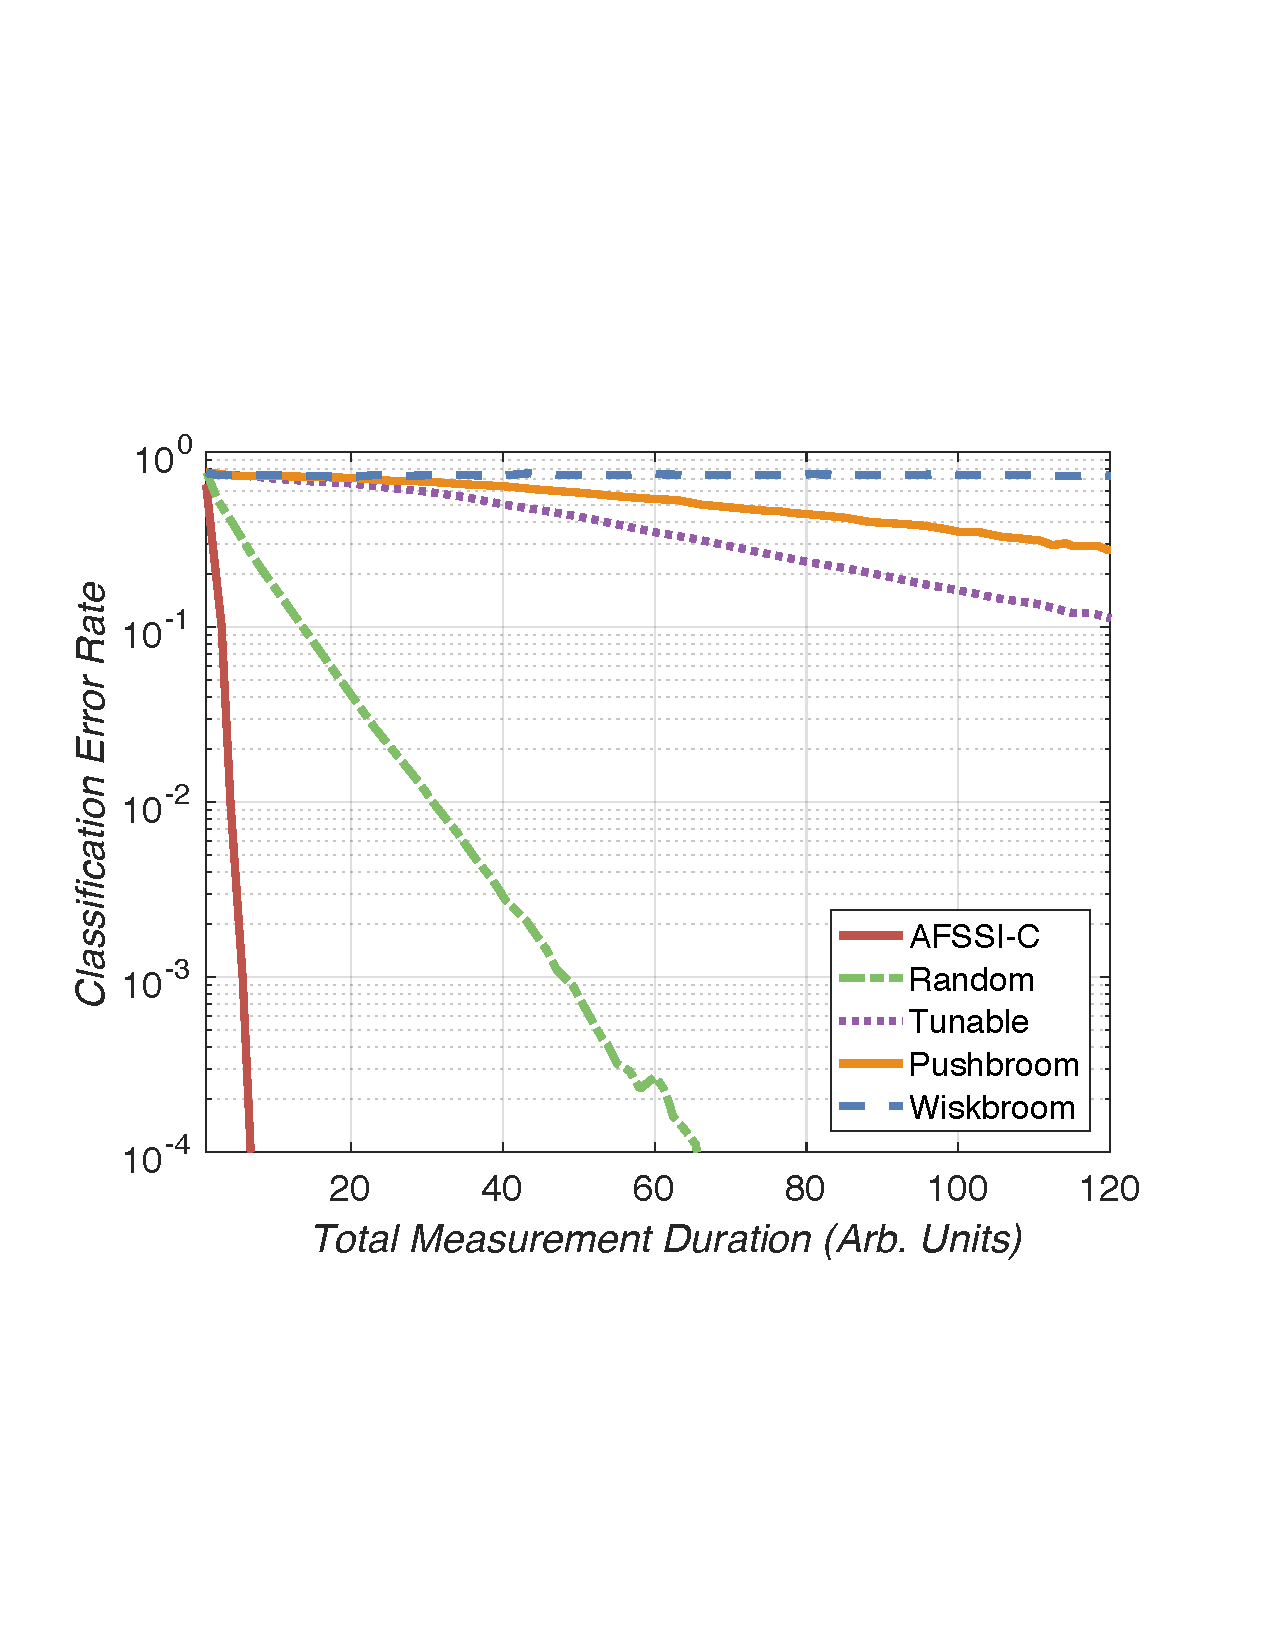
\includegraphics[scale=0.85]{afssicVsOtherSpectromers}\\
  \caption{Simulation comparing the classification performance for different measurements at TSNR = 0 for different systems: the \gls{afssi-c} with designed features (joint pPCA), the \gls{afssi-c} with random features, the traditional pushbroom imager, the traditional tunable filter imager, and the traditional whiskbroom imager. The input is a $64 \times 64 \times 38$ spectral datacube with a 4-class library.} \label{fig:afssicVsOtherSpectromers}
\end{figure}
%
There are a number of phenomena which give the \gls{afssi-c} an advantage over traditional systems. When comparing the \gls{afssi-c} system with joint-pPCA designed features to traditional systems at the 5\textsuperscript{th} measurement in \Cref{fig:afssicVsOtherSpectromers}, we see that the classification accuracy improves by 250$\,\times$. This improvement in performance is attributed to a combination of factors such as the open aperture architecture of the \gls{afssi-c} design, lack of scanning, and adaptivity. 

\Cref{fig:afssicVsOtherSpectromers} also demonstrates the advantage joint-pPCA. By inspecting the 5th measurement, one can observe a 100$\,\times$ performance gain relative to static, pseudo-random coding. The performance curve for the random coding case is generated by directly classifying from the acquired measurements using an identical Bayesian inference framework. The information processing inequality of information theory~\cite{cover2012elements} guarantees us that the alternative approach of classifying after datacube reconstructions can do no better than direct classification. Thus, the difference of these two curves represents the actual classification performance improvement due to adaptivity, while the separation between the static-coded curve and the traditional systems represents the performance improvement arising from the increased open aperture. The simulated results show that the \gls{afssi-c} system to outperform traditional systems where classification is the desired result of the analysis.


\section{Conclusion}

In this chapter, I discussed the \acrfull{afssi-c}, a spectral imager classifier that utilizes adaptive spectral features in a low \acrfull{swap-c} configuration. My collaborators and I were able to show multiple order-of-magnitude improvement in classification accuracy compared to traditional spectral imaging systems when the noise in the system is equal to the minimum separation between the library spectra, by employing a system simulation corroborated with experimental results. By taking advantage of its adaptiveness, the \gls{afssi-c} performance with designed features also achieves multiple order-of-magnitude improvement over a random feature implementation. These adaptive features are designed via Bayesian inference and a novel joint-probabilistic PCA approach, which drives the measurement decision evolution to boost the discrimination ability between spectra candidates at every spatial location. 

Direct classification is a useful modality for many of the applications of spectral imaging. By making measurements of an encoded datacube instead of explicit measurement of every element, huge performance gains are realized. It is reasonable to imagine the \gls{afssi-c} system being of great benefit to a number of industries that rely on \textit{in situ} material classification. 